\documentclass[11pt]{article}

\usepackage[T1]{fontenc}
\usepackage[utf8]{inputenc}
\usepackage{lmodern}
\usepackage[margin=0.82in]{geometry}
\usepackage{amsmath,amssymb}
\usepackage{booktabs}
\usepackage{longtable}
\usepackage{tabularx}
\usepackage{array}
\usepackage{graphicx}
\usepackage{float}
\usepackage[section]{placeins}
\usepackage{caption}
\usepackage{subcaption}
\usepackage{enumitem}
\usepackage{xcolor}
\usepackage{microtype}
\usepackage{setspace}
\usepackage{fancyhdr}
\usepackage{hyperref}
\usepackage{url}

\definecolor{projectblue}{HTML}{2878B5}
\definecolor{projectred}{HTML}{D95F45}
\definecolor{projectgreen}{HTML}{1B9E77}
\definecolor{lightgray}{HTML}{F1F3F5}
\definecolor{darkgray}{HTML}{3B4650}

\hypersetup{
  colorlinks=true,
  linkcolor=projectblue,
  citecolor=projectblue,
  urlcolor=projectblue,
  pdftitle={Analysis of the Velocity, Integration-Time, Beam-Support, and Flow-Reversal Synthetic INR Pilot},
  pdfauthor={UAI PostDoc INR--Radar Project}
}

\pagestyle{fancy}
\fancyhf{}
\lhead{UAI PostDoc INR--Radar Project}
\rhead{Synthetic Pilot Results}
\cfoot{\thepage}
\setlength{\headheight}{14pt}
\setstretch{1.06}
\setlist[itemize,enumerate]{leftmargin=*}
\setlist[description]{style=nextline}
\captionsetup{font=small,labelfont=bf}
\graphicspath{{figures/}}

\newcommand{\Ne}{N_{\mathrm e}}
\newcommand{\Te}{T_{\mathrm e}}
\newcommand{\Ti}{T_{\mathrm i}}
\newcommand{\nrmse}{\mathrm{NRMSE}}
\newcommand{\kmps}{\mathrm{km\,s^{-1}}}
\newcommand{\dex}{\mathrm{dex}}
\newcommand{\targetreg}{\texttt{xy030\_t030}}
\newcommand{\dataonly}{\texttt{data\_only}}

\title{\textbf{Analysis of the Velocity, Integration-Time, Beam-Support,\\
and Flow-Reversal Synthetic INR Pilot}\\[0.6em]
\large Implications for SIREN Regularization, Validation, and the Transition to Real ISR Data}
\author{Prepared for the UAI PostDoc INR--Radar Project}
\date{July 2026}

\begin{document}

\maketitle

\begin{center}
\colorbox{lightgray}{%
\begin{minipage}{0.92\textwidth}
\textbf{Evaluation contract.}
The reconstruction target in this report is the plasma field represented by the radar data product.
For a synthetic measurement with a finite integration interval, the corresponding integration-averaged
synthetic field is the ground truth. The INR is not penalized for failing to recover an unavailable
instantaneous midpoint field. Integration time is metadata describing the measurement, not a defect in
SIREN and not a model-ranking penalty.
\end{minipage}}
\end{center}

\begin{abstract}
This report analyzes 18 completed SIREN-based implicit neural representation (INR) runs designed to
test electron-density reconstruction from sparse radar-like measurements. The pilot contains nine
synthetic observation cases, each trained as a data-only model and as a model with adaptive horizontal
and temporal curvature regularization. The ordinary cases vary beam support (42 or 23 locations),
horizontal speed (0.36 or $2.00~\kmps$), and integration time (1 or 10 minutes). A ninth case represents
a rare flow-reversal configuration with two elongated plasma structures moving in opposite directions,
23 beams, $1.00~\kmps$ speeds, and a 2-minute integration.

The main result is favorable for the current SIREN baseline. The regularized model improves active-region
error against the radar-integrated synthetic truth in all nine cases, with a mean density-RMSE reduction of
49.2\%. The regularized 42-beam ordinary cases achieve active-region normalized RMSE between 4.7\% and
7.4\%; the 23-beam cases achieve 12.4\% to 17.3\%. Beam support is the dominant experimental factor:
42 beams reduce active-region density RMSE by 40.7\% on average across matched configurations and both
training modes. The flow-reversal case is more difficult, but regularization improves normalized RMSE from
47.5\% to 30.3\%, full-field correlation from 0.847 to 0.971, and active-gradient RMSE by 42.0\%.

No run exhibits spatial or temporal curvature collapse. However, a loss-controller limitation is identified:
all 10-minute regularized cases reach the configured temporal-lambda ceiling of $10^{-6}$ while attaining a
temporal/reference-loss ratio of only about 0.01 rather than the requested 0.30. Consequently, those runs
demonstrate successful reconstruction with the implemented regularization, but they do not constitute a
controlled test of a 0.30 temporal-loss ratio. The report concludes that synthetic data remain valuable as
a diagnostic and truth-known validation environment, but should no longer be the main source of project
evidence. The recommended next milestone is a paired real/semi-synthetic experiment based on one well-supported
42-beam ISR event, using actual coordinates, timestamps, integration products, formal uncertainties, quality
flags, and withheld-beam/time validation.
\end{abstract}

\tableofcontents
\listoffigures
\listoftables
\newpage

\section{Purpose and Decision Context}

The project objective is to reconstruct continuous ionospheric plasma fields from sparse multi-beam
incoherent scatter radar (ISR) products while communicating where those reconstructions are reliable.
The current implementation uses a sine-activated coordinate network inspired by SIREN
\cite{Sitzmann2020SIREN}. It maps horizontal position and time to log electron density,
\begin{equation}
  f_{\theta}(x,y,t) \approx \log_{10}\Ne(x,y,t),
\end{equation}
and uses derivatives of the continuous field to impose spatial and temporal soft priors.

The pilot was designed to answer five practical questions.
\begin{enumerate}
  \item Does moderate curvature regularization improve interpolation between sparse beam locations?
  \item How strongly does performance depend on 42 versus 23 sampled locations?
  \item Does the current baseline remain usable when the represented plasma pattern moves rapidly?
  \item Can the model represent a rare two-sided flow-reversal morphology without collapsing to a single
  smooth structure?
  \item Do the curvature terms and adaptive loss controller behave as intended, or do they become zero,
  saturate, or lose influence?
\end{enumerate}

This analysis is intended to guide the next research action. It is not a claim that the pilot spans the
full ISR error model, full 4D geometry, or all relevant plasma morphologies. The central decision is whether
to invest next in a larger idealized synthetic matrix, in alternative INR architectures, or in real-data and
semi-synthetic validation.

\section{Correct Definition of the Reconstruction Target}

\subsection{Radar Products Define the Available Target}

For an integration interval $T_i$ centered at timestamp $t_i$, a simplified density observation model is
\begin{equation}
  y_i = \frac{1}{T_i}\int_{t_i-T_i/2}^{t_i+T_i/2}
  \Ne(\mathbf r_i,\tau)\,\mathrm d\tau + \epsilon_i,
  \label{eq:integration}
\end{equation}
where $\mathbf r_i$ denotes the sampled position and $\epsilon_i$ collects statistical fitting error and
other measurement effects. Real ISR processing is more complex than direct scalar averaging because plasma
parameters are inferred from integrated spectra, but Equation~\eqref{eq:integration} captures the synthetic
observation operator used in this pilot and the essential fact that a finite-integration product represents
an interval, not an instantaneous sample \cite{LehtinenHuuskonen1996,Virtanen2008,Diaz2026ISRError}.

The project cannot control the integration products already delivered by a radar archive. It may sometimes
be possible to request reprocessing at shorter integration times, at the cost of larger fitting uncertainty,
but this is an acquisition and processing tradeoff rather than an INR architecture property. The appropriate
modeling objective is therefore
\begin{equation}
  f_{\theta}(x,y,t_i) \approx \log_{10}\overline{\Ne}_{T_i}(x,y,t_i),
\end{equation}
where $\overline{\Ne}_{T_i}$ is the field represented by that radar product.

\subsection{What Is Excluded from Model Selection}

The synthetic generator stores both the integration-averaged truth and the instantaneous field at the
integration midpoint. The latter is useful for understanding the observation operator, but it is not used
to rank SIREN, select regularization weights, or compare integration products. A model should not be labeled
unsuccessful because it cannot infer information that is absent from its inputs.

Accordingly, all principal results in this report use:
\begin{itemize}
  \item error against the radar-integrated synthetic truth;
  \item spatial correlation with that same truth;
  \item gradient error for that same represented field;
  \item held-support interpretation through beam geometry;
  \item curvature and loss-controller diagnostics.
\end{itemize}

The different integration cases are also not treated as identical targets. A smoother 10-minute product may
be easier to interpolate than a 1-minute product. Lower error in the 10-minute case does not imply that the
radar product is more physically informative; it only describes reconstruction of the available product.

\section{Experimental Design}

\subsection{Synthetic Field and Observation Geometry}

The ordinary synthetic field is a high-amplitude moving Gaussian-like electron-density enhancement on a
$500~\mathrm{km}\times 500~\mathrm{km}$ horizontal domain. Its baseline density is $10^9~\mathrm{m^{-3}}$
and its enhancement reaches approximately $10^{12}~\mathrm{m^{-3}}$. The model target is
$\log_{10}\Ne$. Measurements are created at fixed synthetic beam locations and at the timestamps appropriate
to each product.

The flow-reversal case contains two elongated enhancements centered on opposite sides of a horizontal
boundary. One translates in the positive $x$ direction and the other in the negative $x$ direction, each at
$1.00~\kmps$. This is not intended to estimate the occurrence rate of such events. It is a deliberately rare
stress test of whether a globally smooth coordinate network can preserve two nearby structures with opposing
kinematics.

\begin{table}[H]
\centering
\caption{Nine synthetic observation cases. Each case was trained twice, producing 18 runs.}
\label{tab:cases}
\small
\begin{tabular}{llrrrr}
\toprule
Family & Geometry & Beams & Speed [$\kmps$] & Integration [min] & Time records \\
\midrule
Ordinary patch & sparse grid & 42 & 0.36 & 1 & 21 \\
Ordinary patch & sparse grid & 42 & 0.36 & 10 & 3 \\
Ordinary patch & sparse grid & 42 & 2.00 & 1 & 21 \\
Ordinary patch & sparse grid & 42 & 2.00 & 10 & 3 \\
Ordinary patch & sparse 23 & 23 & 0.36 & 1 & 21 \\
Ordinary patch & sparse 23 & 23 & 0.36 & 10 & 3 \\
Ordinary patch & sparse 23 & 23 & 2.00 & 1 & 21 \\
Ordinary patch & sparse 23 & 23 & 2.00 & 10 & 3 \\
Flow reversal & sparse 23 & 23 & $\pm 1.00$ & 2 & 11 \\
\bottomrule
\end{tabular}
\end{table}

\subsection{Training Configurations}

Every case was trained for 15,000 steps under two configurations:
\begin{description}
  \item[Data only.] The objective contains only the measured-point data loss. Fixed diagnostic collocation
  points remain active, so derivative behavior is measured even though it is not optimized.
  \item[\targetreg.] The objective uses the same data loss plus horizontal Hessian-curvature and temporal
  second-derivative penalties. A reference-ratio controller attempts to maintain each weighted regularization
  component at 0.30 of a stabilized data-loss reference.
\end{description}

The regularized objective is
\begin{equation}
  \mathcal L = \mathcal L_{\mathrm{data}}
  + \lambda_{xy}\mathcal L_{xy}
  + \lambda_t\mathcal L_t,
\end{equation}
with
\begin{align}
  \mathcal L_{xy} &= \mathbb E_{\mathcal C}
  \left[f_{xx}^2 + 2f_{xy}^2 + f_{yy}^2\right], \\
  \mathcal L_t &= \mathbb E_{\mathcal C}\left[f_{tt}^2\right],
\end{align}
where $\mathcal C$ is the collocation set. The implementation tracks raw and weighted terms, lambda values,
achieved reference ratios, derivative root-mean-square values, derivative near-zero fractions, and parameter
gradient norms. This monitoring is essential because a small regularization loss can mean either a smooth
learned solution or a collapsed derivative pathway.

\subsection{Dense Evaluation and Event-Aware Metrics}

Every trained model was evaluated on a $250\times250$ full-domain grid. The initial analysis saved the first,
middle, and last frames. The main event-aware summary uses the central frame at $t=600~\mathrm{s}$ because the
fast $2~\kmps$ patch lies outside the $500~\mathrm{km}$ domain at the first and last selected frames. Including
those empty-background frames in a mean makes fast cases appear artificially easy.

The active region is defined by
\begin{equation}
  \Omega_{\mathrm{active}} = \{(x,y):\Ne{}_{\mathrm{true}}(x,y,t)>10^{10}~\mathrm{m^{-3}}\}.
\end{equation}
The principal normalized density error is
\begin{equation}
  \nrmse_{\mathrm{active}} =
  \frac{
  \sqrt{\frac{1}{|\Omega_{\mathrm{active}}|}
  \sum_{j\in\Omega_{\mathrm{active}}}(\widehat{\Ne}{}_j-\Ne{}_j)^2}}
  {\sqrt{\frac{1}{|\Omega_{\mathrm{active}}|}
  \sum_{j\in\Omega_{\mathrm{active}}}(\Ne{}_j-10^9)^2}}.
  \label{eq:nrmse}
\end{equation}
This normalization reduces the misleading effect of comparing a high-amplitude compact target with a
lower-amplitude integrated target. Additional metrics include full-domain correlation, active-region bias,
combined first-derivative RMSE, peak recovery relative to the radar-integrated truth, and measured-point
training error.

\section{Results}

\subsection{Run Completion and Curvature Health}

All 18 runs completed 15,000 steps and produced final checkpoints and complete training histories. No run
was flagged as spatially or temporally collapsed. Tail derivative near-zero fractions remained below the
collapse threshold, and the RMS values of $f_{xx}$, $f_{xy}$, $f_{yy}$, and $f_{tt}$ remained nonzero.

This is an important positive result. Performance differences are not explained by one model failing to
learn derivatives. The diagnostic changes previously added to the data-only branch were necessary: without
them, a data-only model could have appeared free of curvature artifacts simply because its derivatives were
not being measured.

\subsection{Primary Reconstruction Results}

Table~\ref{tab:mainresults} reports the event-frame metrics that should drive interpretation. Regularization
reduces active-region density error in every case. The strongest ordinary result is the 42-beam,
$0.36~\kmps$, 1-minute case, with 4.7\% normalized RMSE and 0.999 spatial correlation. The 42-beam
$2.00~\kmps$ cases remain between 5.3\% and 7.4\%. The 23-beam ordinary cases are less accurate but remain
between 12.4\% and 17.3\% after regularization.

\begin{table}[H]
\centering
\caption{Event-frame reconstruction against radar-integrated synthetic truth. Improvements are relative
to the data-only run for the same observation case.}
\label{tab:mainresults}
\scriptsize
\resizebox{\textwidth}{!}{%
\begin{tabular}{lrrrrrr}
\toprule
Case & Data-only NRMSE [\%] & Regularized NRMSE [\%] & Data corr. & Reg. corr. & Density improv. [\%] & Gradient improv. [\%] \\
\midrule
42 beams, 0.36 $\kmps$, 1 min & 13.0 & \textbf{4.7} & 0.995 & 0.999 & 64.1 & 48.8 \\
42 beams, 0.36 $\kmps$, 10 min & 25.1 & \textbf{5.2} & 0.970 & 0.999 & 79.1 & 48.4 \\
42 beams, 2.00 $\kmps$, 1 min & 15.6 & \textbf{7.4} & 0.989 & 0.998 & 52.3 & $-17.4$ \\
42 beams, 2.00 $\kmps$, 10 min & 22.1 & \textbf{5.3} & 0.980 & 0.999 & 76.2 & 64.9 \\
23 beams, 0.36 $\kmps$, 1 min & 19.1 & \textbf{17.3} & 0.985 & 0.993 & 9.5 & 39.5 \\
23 beams, 0.36 $\kmps$, 10 min & 30.8 & \textbf{14.0} & 0.969 & 0.993 & 54.7 & 42.1 \\
23 beams, 2.00 $\kmps$, 1 min & 16.4 & \textbf{12.4} & 0.993 & 0.996 & 24.6 & 19.2 \\
23 beams, 2.00 $\kmps$, 10 min & 30.1 & \textbf{16.3} & 0.952 & 0.988 & 45.6 & 50.0 \\
Flow reversal, 23 beams, 1.00 $\kmps$, 2 min & 47.5 & \textbf{30.3} & 0.847 & 0.971 & 36.2 & 42.0 \\
\bottomrule
\end{tabular}}
\end{table}

\begin{figure}[H]
\centering
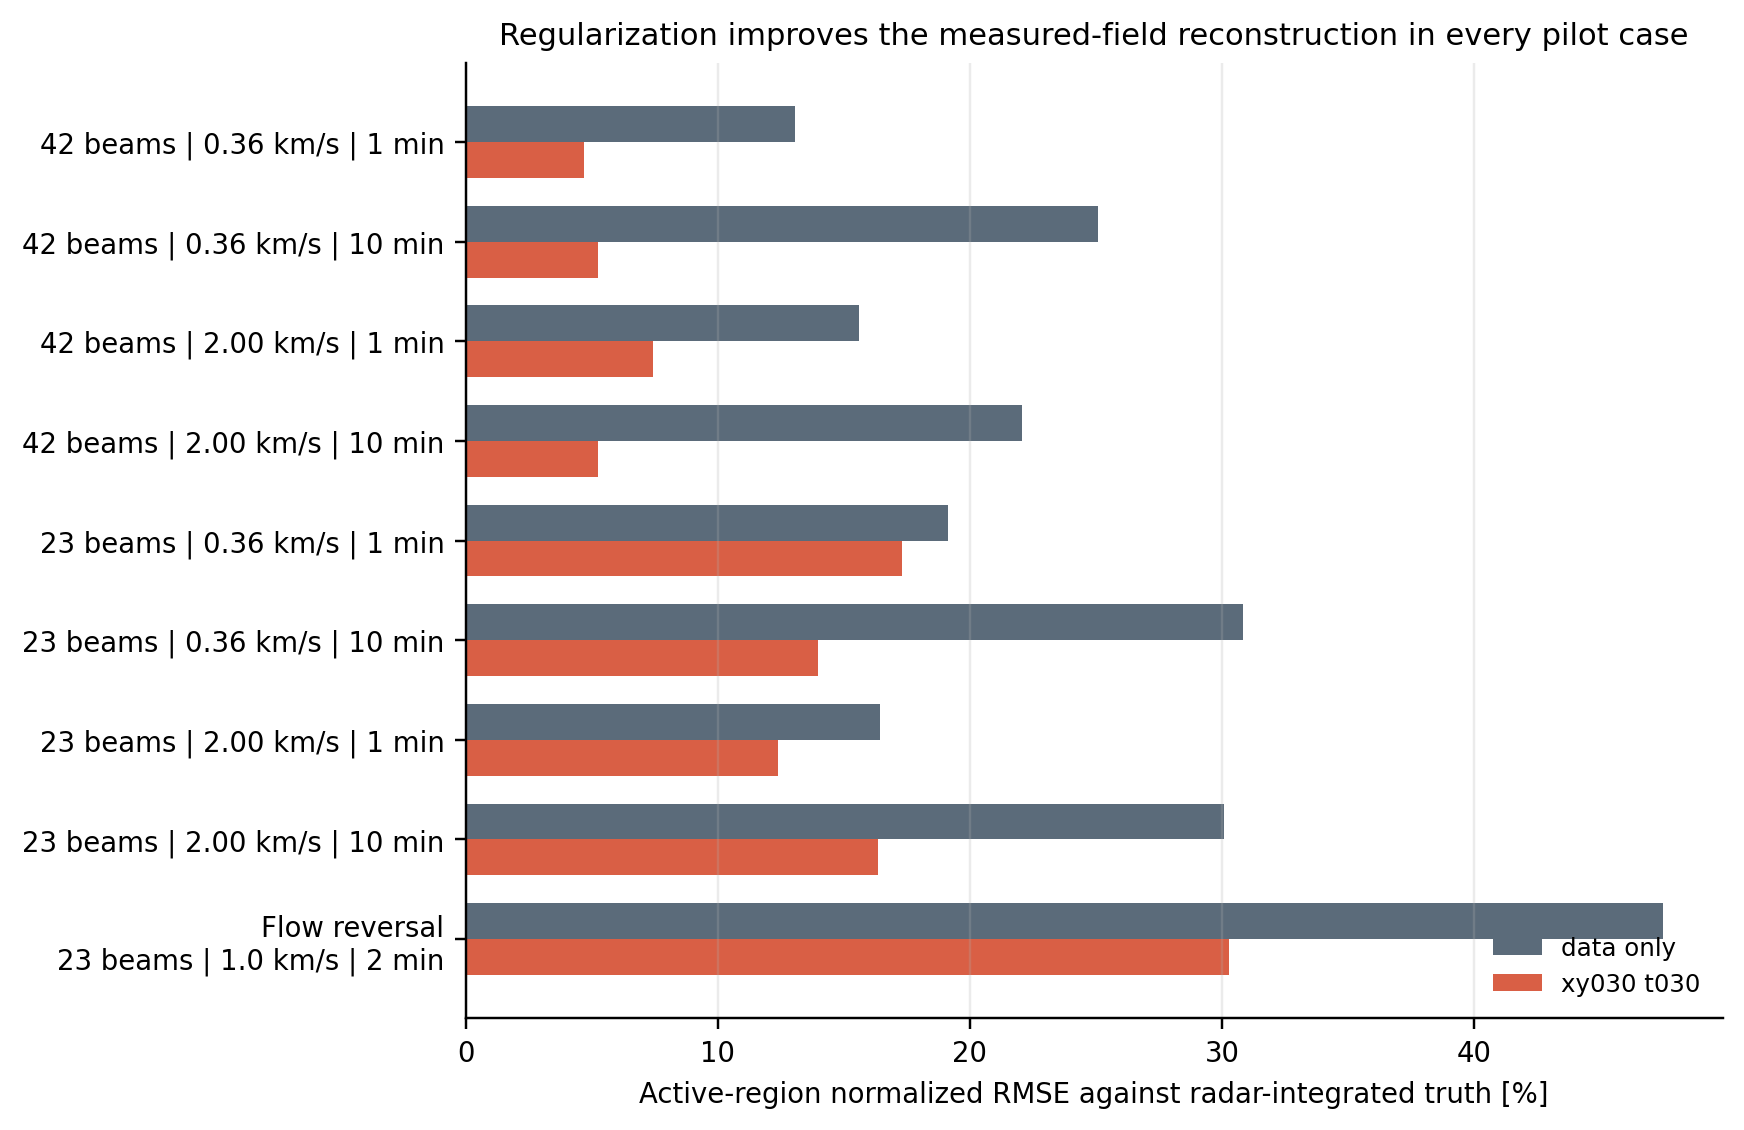
\includegraphics[width=0.96\textwidth]{active_nrmse_by_case.png}
\caption{Active-region normalized RMSE for the data-only and regularized models. The comparison is always
against the radar-integrated synthetic truth corresponding to the measurement product. Regularization
improves all nine cases.}
\label{fig:nrmse}
\end{figure}

\subsection{What the Regularization Result Means}

Across the nine cases, \targetreg{} reduces active-region density RMSE by 49.2\% on average. The range is
9.5\% to 79.1\%. This is stronger evidence than the earlier four-run weight pilot because it spans two beam
supports, two speeds, two integration products, and a flow-reversal morphology.

The result does not yet prove that 0.30/0.30 is globally optimal. It establishes a narrower and useful claim:
the current moderate regularization is consistently preferable to data-only fitting for dense reconstruction
of these radar products. Final lambda selection still requires multiple seeds and withheld real-data tests.

The gradient result is also mostly favorable: active-gradient RMSE improves in eight of nine cases, by 37.5\%
on average. The exception is the 42-beam, $2.00~\kmps$, 1-minute case, where density RMSE improves by 52.3\%
but active-gradient RMSE worsens by 17.4\%. This exception prevents the project from selecting models on
density alone. A reconstruction can be numerically accurate in field value while distorting gradients that
may be scientifically important or later used in derived quantities.

\begin{figure}[H]
\centering
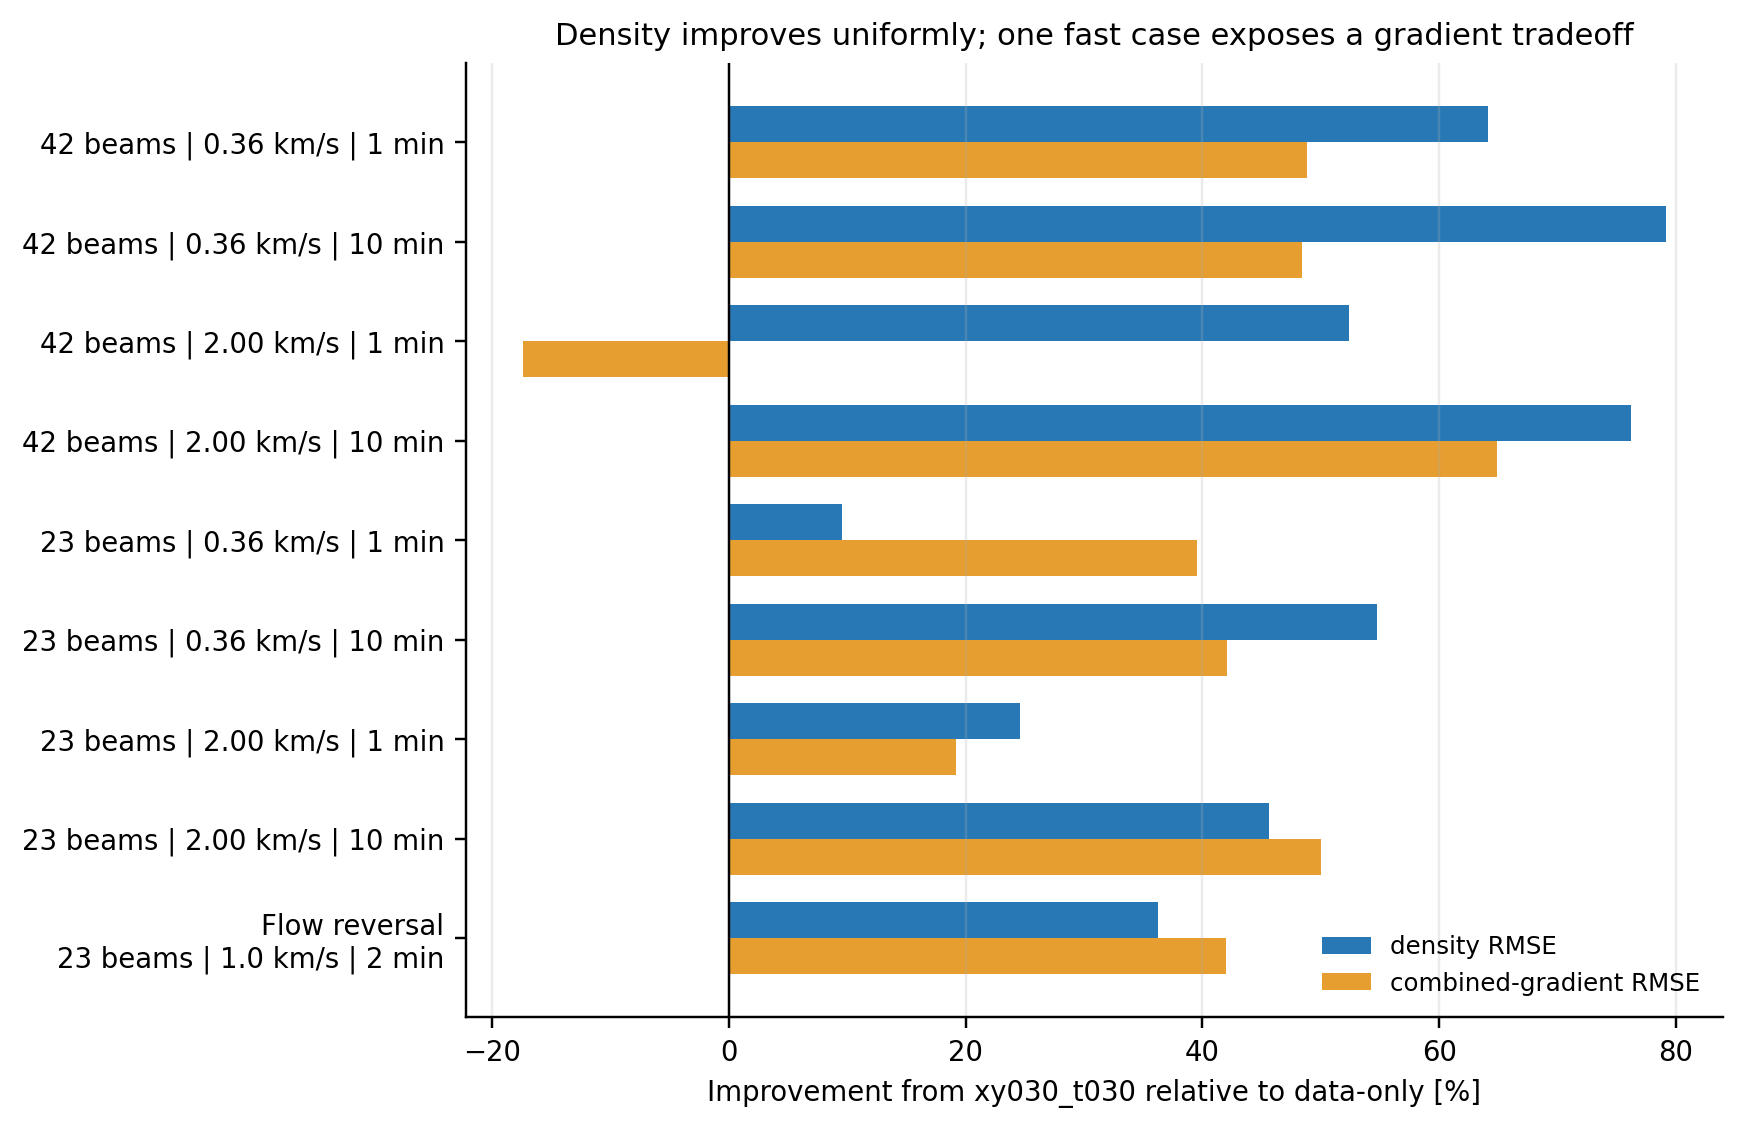
\includegraphics[width=0.96\textwidth]{regularization_improvement.png}
\caption{Percentage improvement produced by \targetreg{} relative to data-only fitting. Positive values
indicate lower error. Density improves uniformly; the negative gradient result in the 42-beam fast 1-minute
case is a targeted warning for future loss selection.}
\label{fig:regimprovement}
\end{figure}

\subsection{Beam Support Is the Dominant Experimental Factor}

Across matched ordinary cases and both training modes, 42 beams reduce active-region density RMSE by 40.7\%
on average relative to 23 beams. The interaction with regularization is especially important. With data-only
training, the average 42-beam advantage is 20.5\%; with \targetreg{}, it is 60.9\%. The prior is most useful
when the observation geometry contains enough distributed support to constrain the smooth solution.

\begin{table}[H]
\centering
\caption{Reduction in active-region density RMSE from using 42 rather than 23 beams.}
\label{tab:beameffect}
\small
\begin{tabular}{rrr}
\toprule
Speed and product & Data-only reduction [\%] & Regularized reduction [\%] \\
\midrule
0.36 $\kmps$, 1 min & 31.8 & 73.0 \\
0.36 $\kmps$, 10 min & 18.6 & 62.5 \\
2.00 $\kmps$, 1 min & 5.0 & 40.0 \\
2.00 $\kmps$, 10 min & 26.6 & 67.9 \\
\midrule
Mean & 20.5 & 60.9 \\
\bottomrule
\end{tabular}
\end{table}

\begin{figure}[H]
\centering
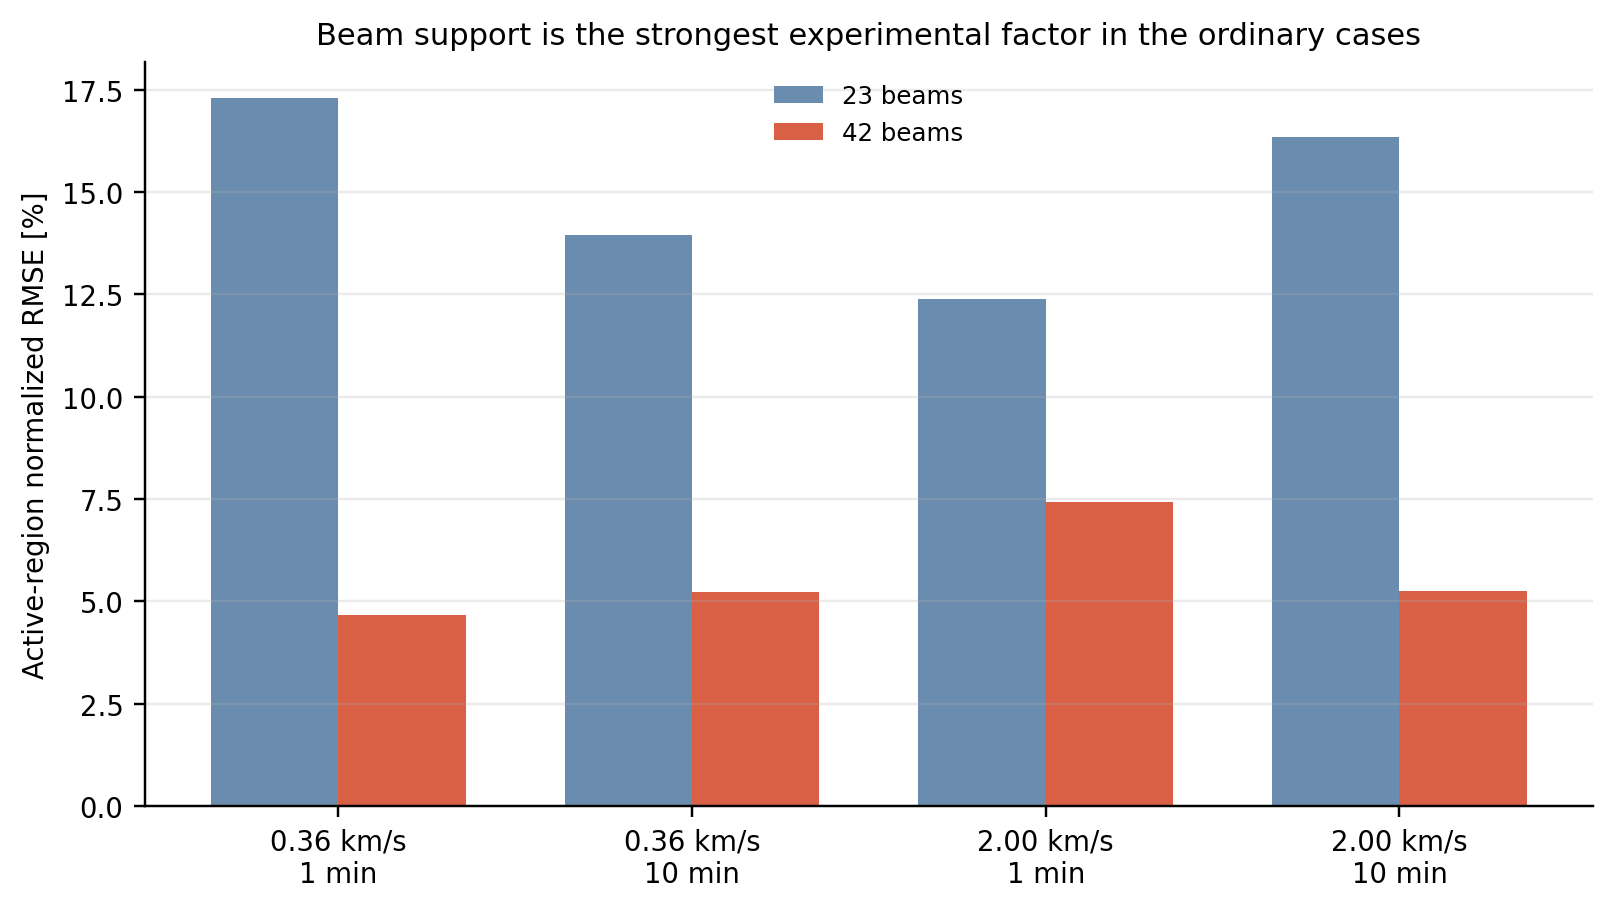
\includegraphics[width=0.85\textwidth]{beam_count_effect.png}
\caption{Regularized active-region normalized RMSE for 23- and 42-beam geometries. The 23-beam cases are
usable but consistently less accurate. Beam count alone is not the complete support description; future
real-data work should also include distances, angular diversity, altitude coverage, and missing records.}
\label{fig:beams}
\end{figure}

The result supports two project decisions. First, the final reliability layer should use geometry/support
features rather than presenting all locations as equally constrained. Second, 11-beam data should be treated
primarily as a reliability and failure-detection test, not as the next reconstruction benchmark. A method
that returns a visually plausible 11-beam field without warning may be less useful than one that correctly
marks large regions as prior dominated.

\subsection{Velocity and Integration Product}

Within the represented radar products, the regularized SIREN remains effective across both velocities and
both integration times. There is no monotonic evidence that the 10-minute product is harder for the INR:
the 42-beam regularized NRMSE values are 4.7\%, 5.2\%, 7.4\%, and 5.3\% across the four ordinary cases.
The corresponding 23-beam values are 17.3\%, 14.0\%, 12.4\%, and 16.3\%.

These values must not be interpreted as evidence that a 10-minute product is physically superior. The target
itself changes with integration. The correct conclusion is that the current INR reconstructs each supplied
synthetic radar product consistently. If the project later receives shorter-integration reprocessed data,
those products should be evaluated on their own fitting uncertainties and withheld-data performance, not
assumed to be preferable solely because they are temporally finer.

\subsection{Sparse Training Error Does Not Select the Best Reconstruction}

All final measured-point RMSE values are below $0.0058~\dex$. Several data-only 10-minute models fit the
sparse observations almost exactly while producing much larger dense error. Table~\ref{tab:trainvsdense}
shows representative examples.

\begin{table}[H]
\centering
\caption{Representative measured-point fit versus dense active-region reconstruction. Smaller training
error does not imply better interpolation.}
\label{tab:trainvsdense}
\small
\begin{tabular}{llrr}
\toprule
Case & Mode & Final training RMSE [dex] & Dense active NRMSE [\%] \\
\midrule
42 beams, 0.36 $\kmps$, 10 min & Data only & $4.50\times10^{-6}$ & 25.1 \\
 & Regularized & $1.42\times10^{-3}$ & \textbf{5.2} \\
42 beams, 2.00 $\kmps$, 10 min & Data only & $1.42\times10^{-7}$ & 22.1 \\
 & Regularized & $1.56\times10^{-3}$ & \textbf{5.3} \\
23 beams, 0.36 $\kmps$, 10 min & Data only & $5.37\times10^{-6}$ & 30.8 \\
 & Regularized & $1.26\times10^{-3}$ & \textbf{14.0} \\
Flow reversal & Data only & $3.40\times10^{-3}$ & 47.5 \\
 & Regularized & $1.11\times10^{-3}$ & \textbf{30.3} \\
\bottomrule
\end{tabular}
\end{table}

\begin{figure}[H]
\centering
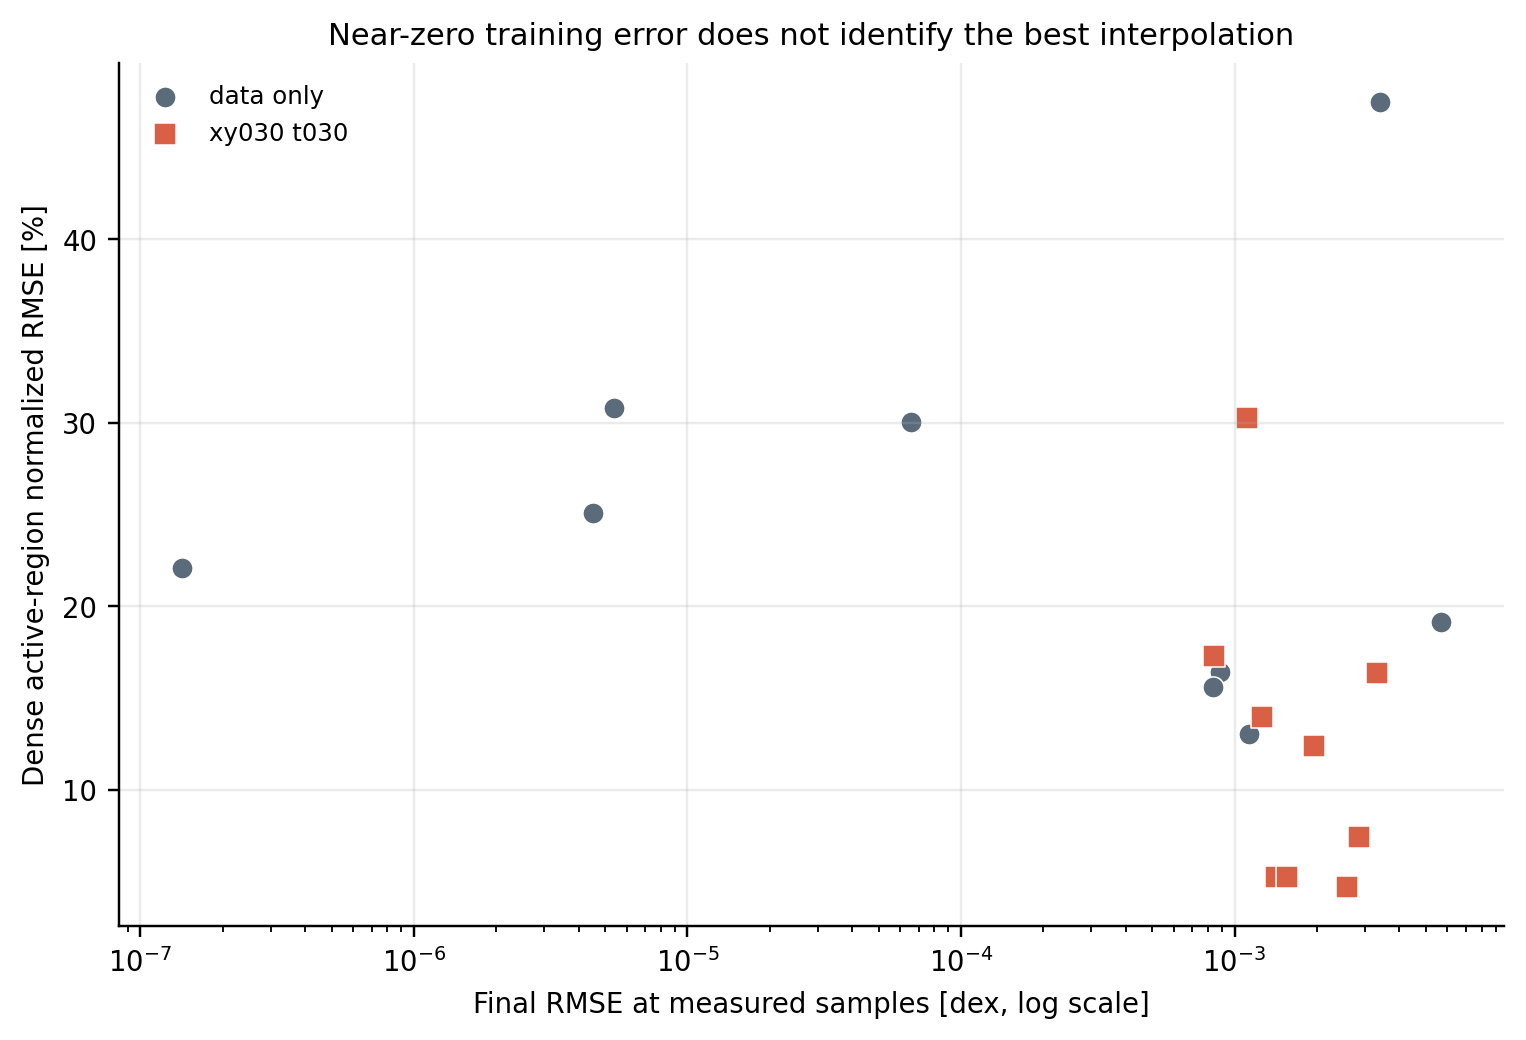
\includegraphics[width=0.78\textwidth]{training_fit_vs_dense_error.png}
\caption{Final measured-point RMSE versus dense event-region error. The horizontal axis is logarithmic.
Near-zero training loss is compatible with poor interpolation, so training loss cannot be the primary
selection criterion.}
\label{fig:trainvsdense}
\end{figure}

This observation directly motivates withheld-beam validation. In real ISR data there is no dense ground
truth, so the closest defensible analogue is to remove measurements with known values, reconstruct them from
the remaining beams, and score the held-out residuals using their formal uncertainties.

\subsection{Flow-Reversal Stress Case}

The flow-reversal case is the most difficult pilot example. Its 23-beam regularized active NRMSE is 30.3\%,
compared with 47.5\% for data-only fitting. Regularization increases full-field correlation from 0.847 to
0.971 and reduces active-gradient RMSE by 42.0\%. Figure~\ref{fig:shearrecon} shows that the model preserves
the broad two-band morphology but fills too much of the central gap and underestimates portions of the
structures.

\begin{figure}[H]
\centering
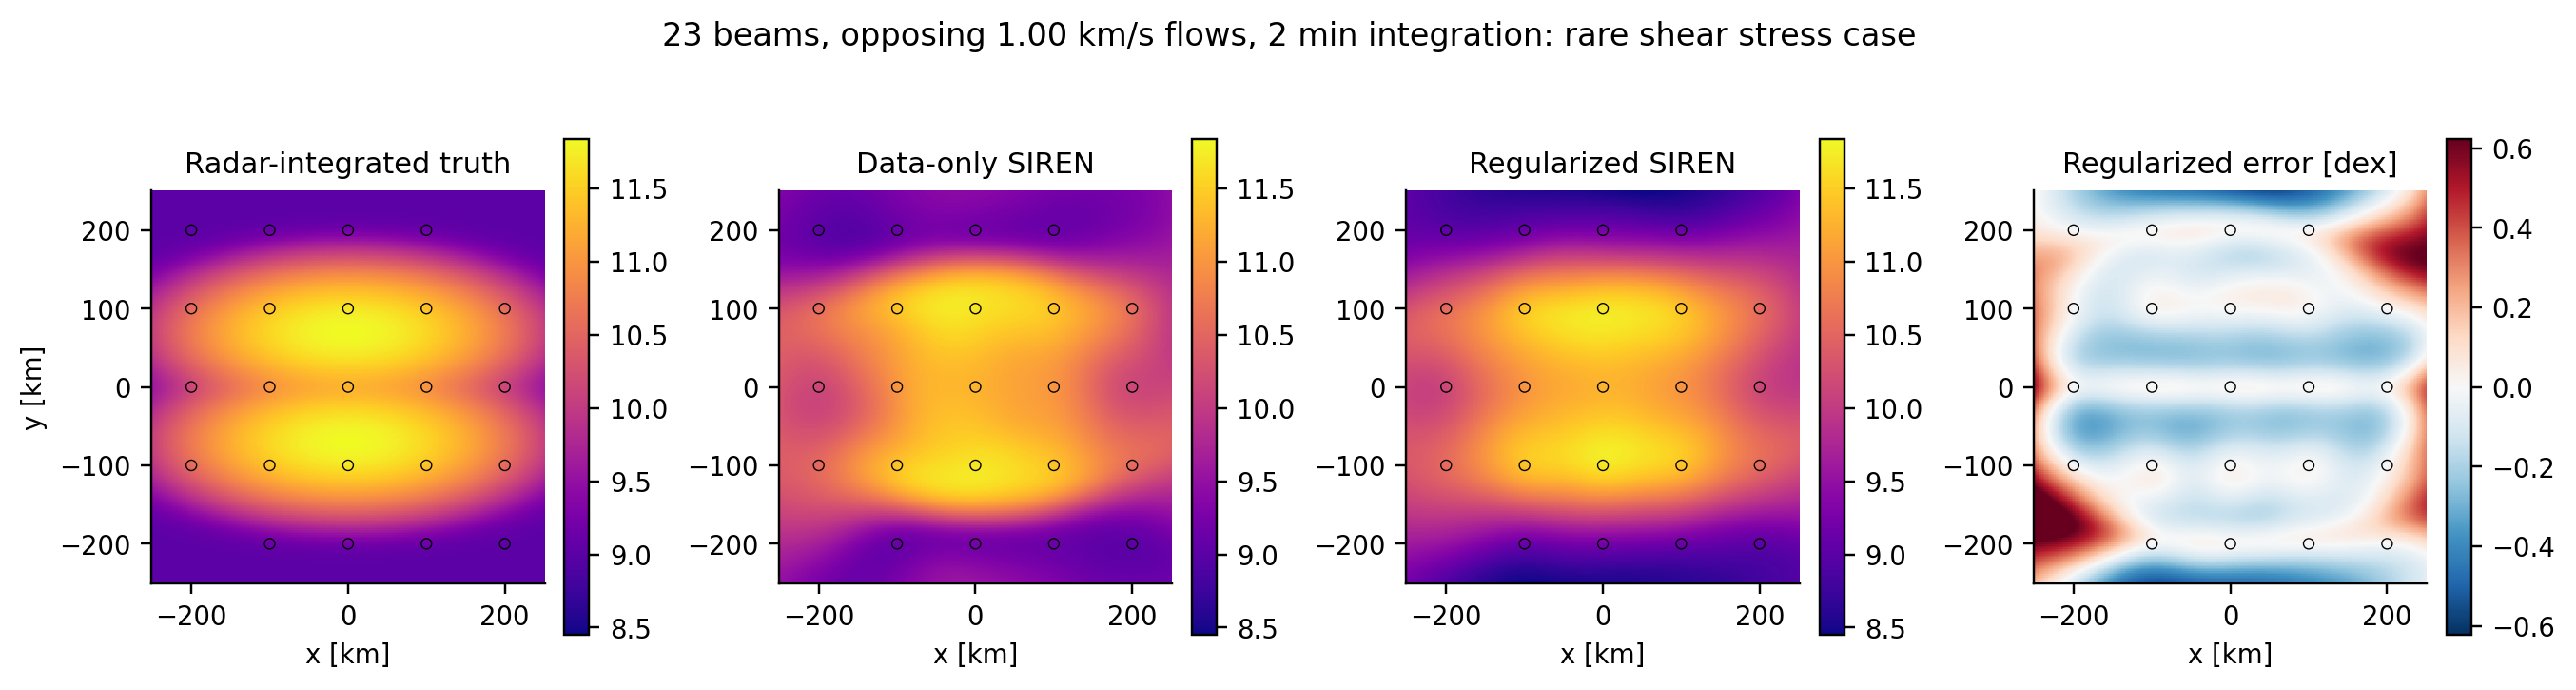
\includegraphics[width=\textwidth]{reconstruction_flow_reversal.png}
\caption{Central frame of the flow-reversal case. Circles mark synthetic beam locations. The regularized
model is smoother and more faithful globally, but the boundary between the bands remains the main error
region. This case should be retained as a rare stress test rather than treated as representative occurrence.}
\label{fig:shearrecon}
\end{figure}

\begin{figure}[H]
\centering
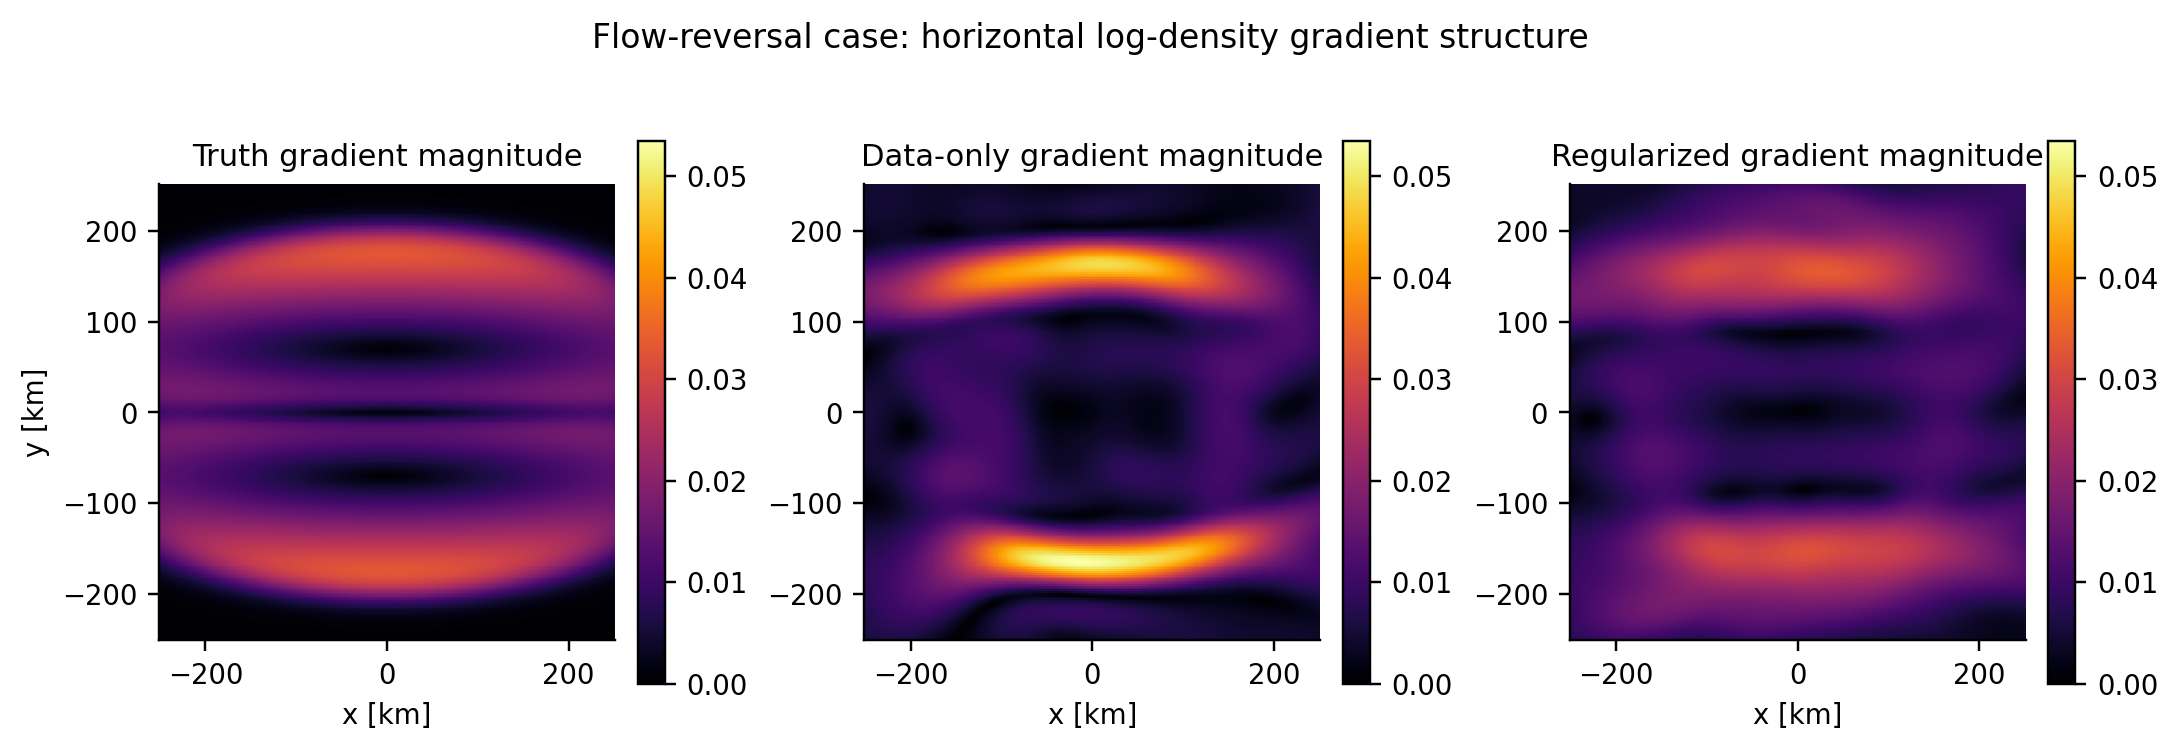
\includegraphics[width=0.94\textwidth]{flow_reversal_gradient_comparison.png}
\caption{Horizontal log-density gradient magnitude for the flow-reversal case. Regularization improves
the band-edge organization, but neither model exactly recovers the gradient structure. A later LOS-velocity
conditioned or local motion-aware model should be compared specifically on this case.}
\label{fig:sheargradient}
\end{figure}

The case does not establish that SIREN is incapable of representing shear. It establishes that sparse density
samples plus global smoothness do not fully constrain the boundary. The next relevant information source is
the radar LOS velocity, not simply a larger density-only network. LOS velocities can initially enter as
conditioning variables, activity/support features, or a separately smoothed horizontal-flow proxy without
turning the project into a full PINN.

\subsection{Loss-Ratio Controller and Curvature Diagnostics}

The spatial reference-ratio controller behaves close to its target. Tail-median spatial ratios generally lie
between 0.275 and 0.329. The temporal controller also reaches approximately 0.27--0.32 for the 1- and 2-minute
cases. In all four 10-minute cases, however, $\lambda_t$ reaches its configured maximum of $10^{-6}$ while the
achieved ratio remains approximately 0.01.

\begin{table}[H]
\centering
\caption{Tail-median regularization diagnostics for the nine \targetreg{} runs.}
\label{tab:lambdas}
\scriptsize
\resizebox{\textwidth}{!}{%
\begin{tabular}{lrrrrr}
\toprule
Case & $\lambda_{xy}$ & $\lambda_t$ & Achieved spatial ratio & Achieved temporal ratio & $f_{tt}$ RMS \\
\midrule
42 beams, 0.36 $\kmps$, 1 min & $4.91\times10^{-8}$ & $8.62\times10^{-8}$ & 0.299 & 0.298 & 5.101 \\
42 beams, 0.36 $\kmps$, 10 min & $5.41\times10^{-8}$ & $1.00\times10^{-6}$ & 0.305 & 0.011 & 0.251 \\
42 beams, 2.00 $\kmps$, 1 min & $2.79\times10^{-7}$ & $8.07\times10^{-10}$ & 0.275 & 0.272 & 56.032 \\
42 beams, 2.00 $\kmps$, 10 min & $6.41\times10^{-8}$ & $1.00\times10^{-6}$ & 0.313 & 0.010 & 0.222 \\
23 beams, 0.36 $\kmps$, 1 min & $6.00\times10^{-8}$ & $1.10\times10^{-7}$ & 0.294 & 0.291 & 4.194 \\
23 beams, 0.36 $\kmps$, 10 min & $5.50\times10^{-8}$ & $1.00\times10^{-6}$ & 0.303 & 0.010 & 0.232 \\
23 beams, 2.00 $\kmps$, 1 min & $3.81\times10^{-7}$ & $1.00\times10^{-9}$ & 0.283 & 0.284 & 47.075 \\
23 beams, 2.00 $\kmps$, 10 min & $1.09\times10^{-7}$ & $1.00\times10^{-6}$ & 0.329 & 0.010 & 0.210 \\
Flow reversal, 23 beams, 2 min & $6.41\times10^{-8}$ & $2.40\times10^{-8}$ & 0.319 & 0.317 & 10.043 \\
\bottomrule
\end{tabular}}
\end{table}

\begin{figure}[H]
\centering
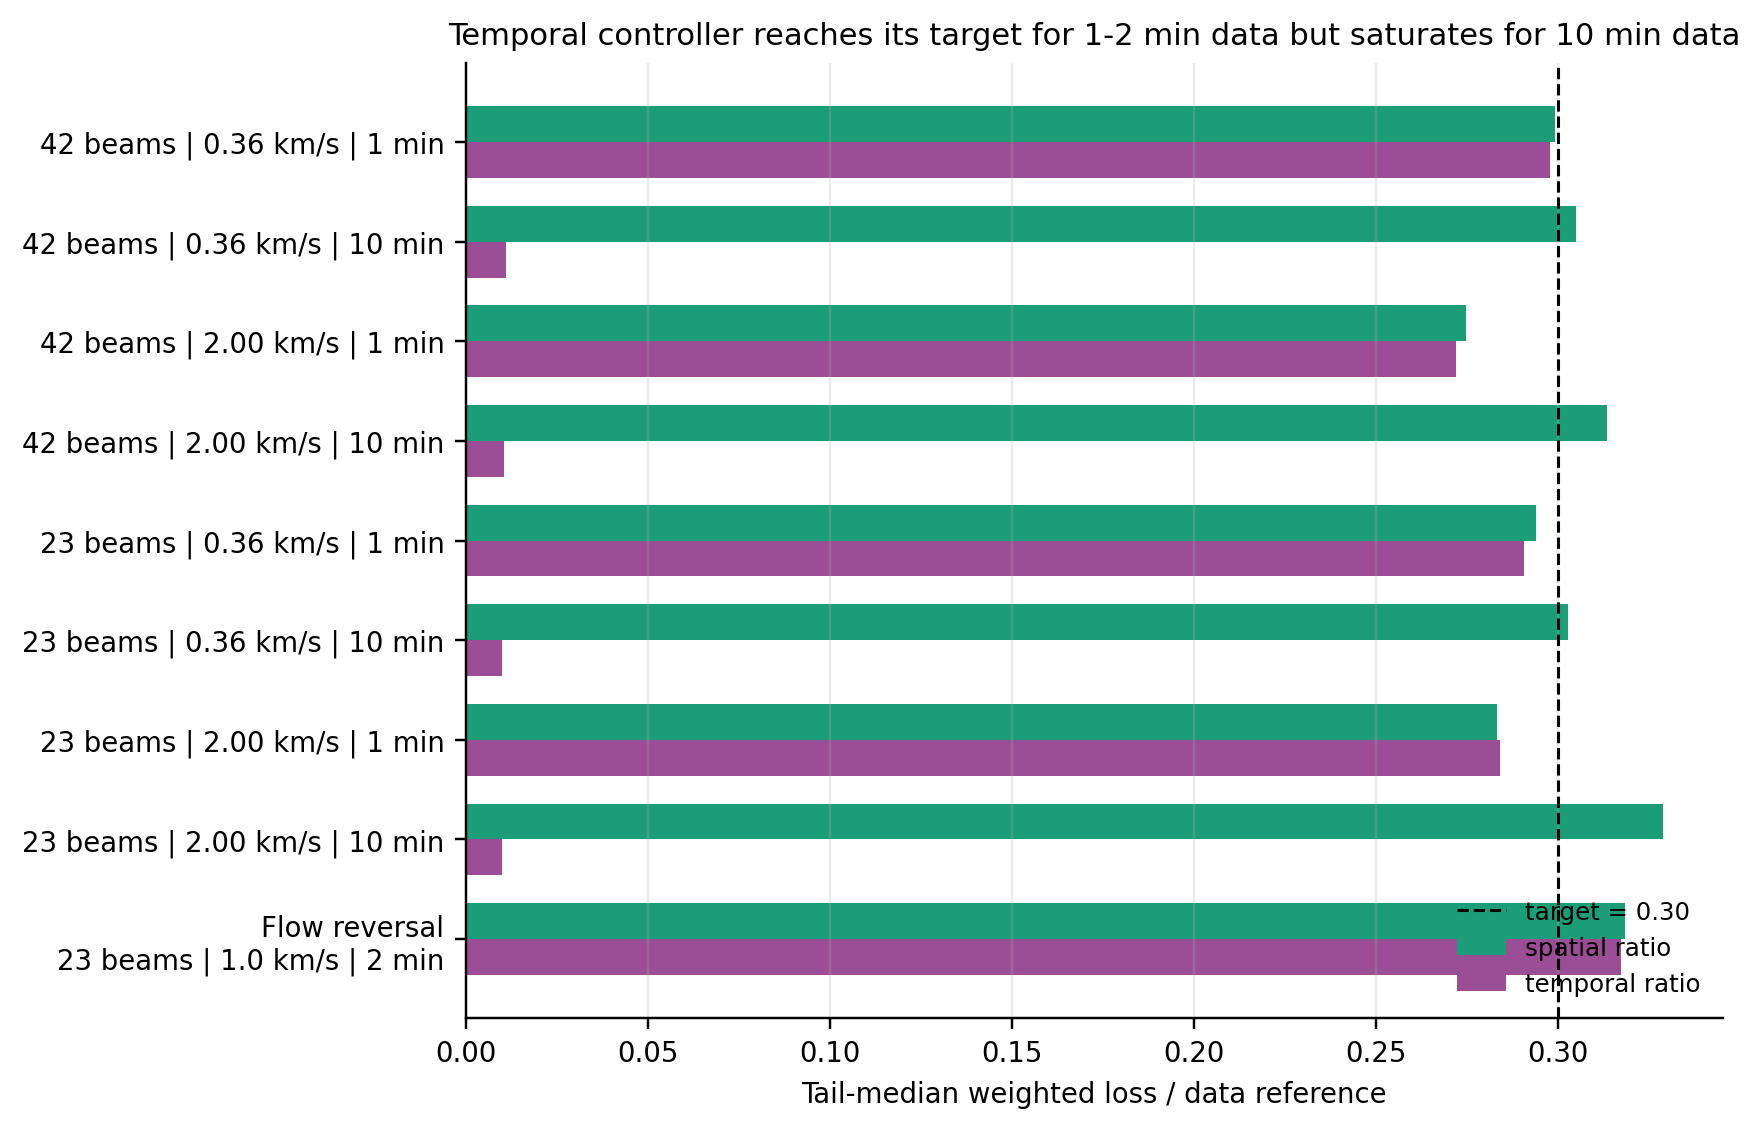
\includegraphics[width=0.96\textwidth]{achieved_loss_ratios.png}
\caption{Tail-median weighted regularization terms relative to the stabilized data-loss reference. The
dashed line is the requested 0.30 ratio. The temporal controller is capped in every 10-minute case.}
\label{fig:lossratios}
\end{figure}

The low temporal ratio is not curvature collapse: $f_{tt}$ remains nonzero. It means the controller cannot
raise the weighted temporal term to its requested fraction under the configured lambda ceiling. Three
interpretations must be separated:
\begin{enumerate}
  \item the 10-minute targets are smoother and therefore have lower raw temporal curvature;
  \item there are only three time records, limiting what a temporal prior can be validated against;
  \item the fixed lambda maximum is not scale invariant across observation products.
\end{enumerate}

The correct next action is not to increase the cap blindly. A focused experiment should vary the cap and
target ratio while monitoring withheld-time error, density error, gradient error, and whether the prediction
becomes prior dominated. Adaptive multi-objective methods such as GradNorm or SoftAdapt may be useful
comparators, but they should be evaluated against this explicit reference-ratio baseline rather than adopted
without a project-specific criterion \cite{Chen2018GradNorm,Heydari2019SoftAdapt,Kendall2018MultiTask}.

\section{Representative Reconstruction Maps}

\subsection{Well-Supported Reference Case}

Figure~\ref{fig:42slow} demonstrates the strongest ordinary case. The regularized reconstruction restores
the peak and radial shape more faithfully than the data-only model. Its active-region NRMSE is 4.7\%, its
spatial correlation is 0.999, and its predicted peak is approximately 96\% of the radar-integrated truth.

\begin{figure}[H]
\centering
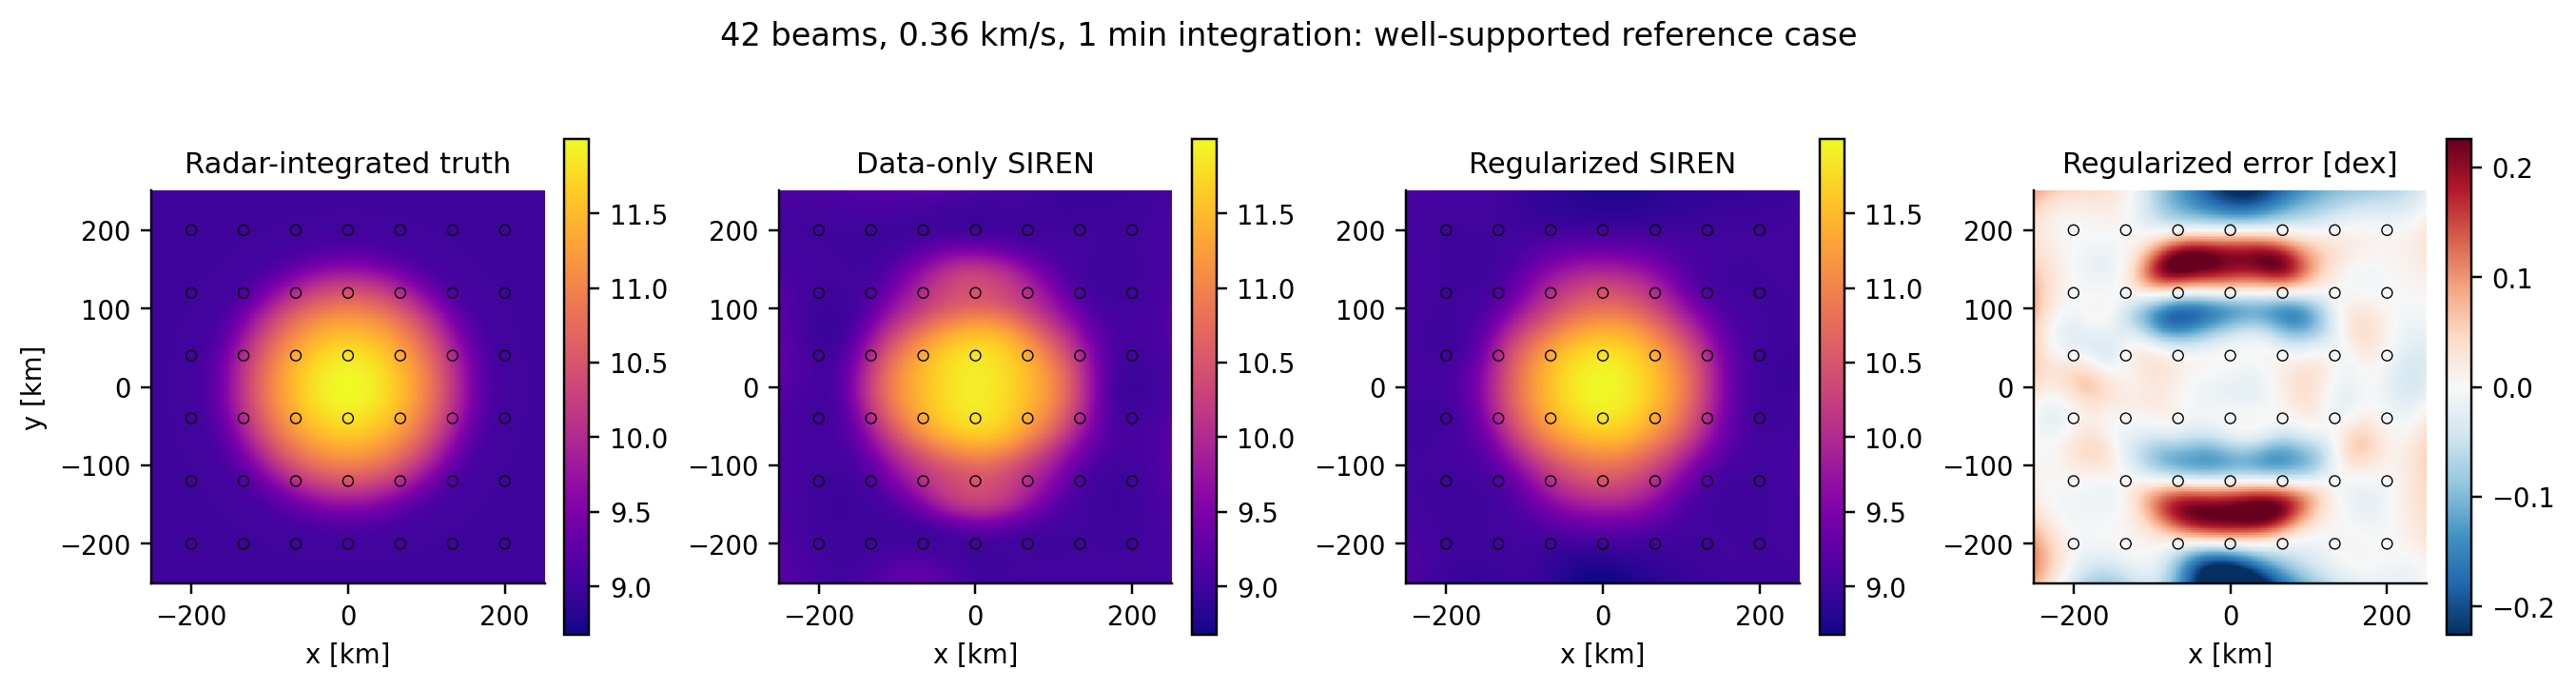
\includegraphics[width=\textwidth]{reconstruction_42_slow_1m.png}
\caption{42 beams, $0.36~\kmps$, 1-minute integration. The error panel is in log-density dex and is clipped
to robust percentiles for visual legibility.}
\label{fig:42slow}
\end{figure}

\subsection{Support-Limited Counterpart}

Reducing the geometry to 23 points increases regularized active NRMSE from 4.7\% to 17.3\% for the same
speed and integration product. Figure~\ref{fig:23slow} shows that the global patch remains identifiable, but
the lower support permits larger amplitude and boundary errors between measurements.

\begin{figure}[H]
\centering
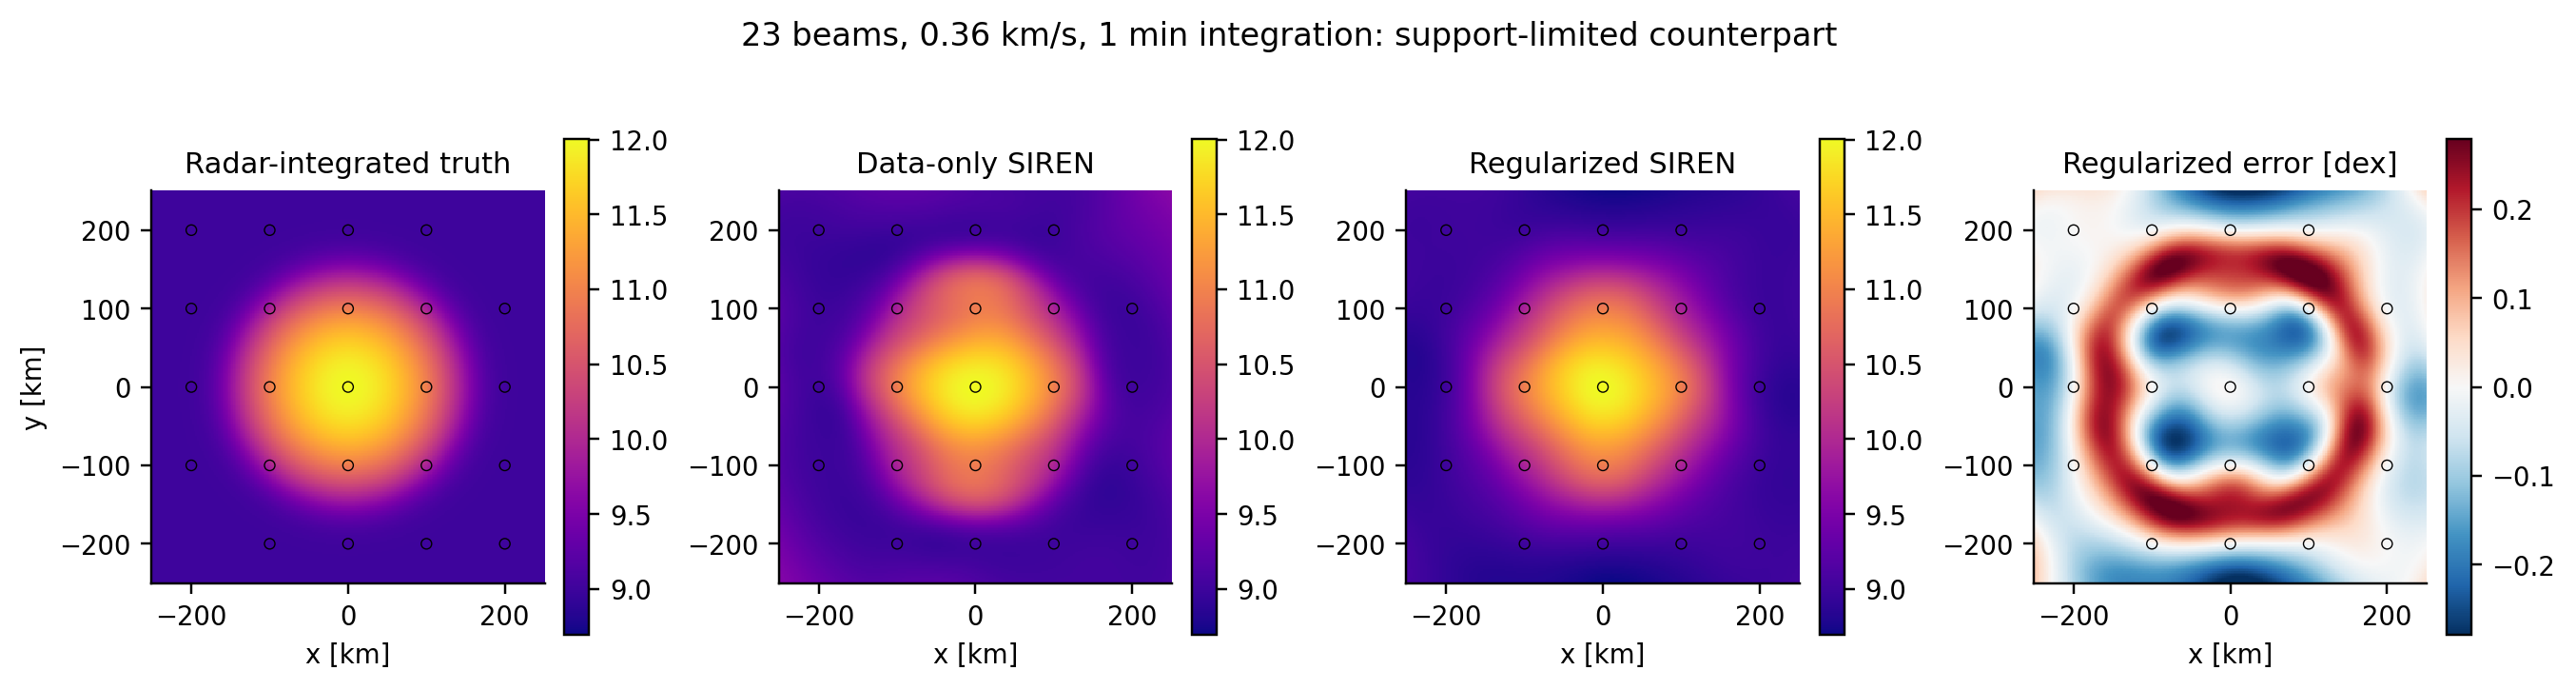
\includegraphics[width=\textwidth]{reconstruction_23_slow_1m.png}
\caption{23 beams, $0.36~\kmps$, 1-minute integration. This paired comparison isolates the effect of
support geometry.}
\label{fig:23slow}
\end{figure}

\subsection{Fast One-Minute Product}

The 42-beam fast case is reconstructed well in density, but it is the one case where the regularized active
gradient RMSE is worse than data only. Figure~\ref{fig:42fast1} shows why both field and derivative metrics
are necessary: visually accurate density does not guarantee the best local derivative field.

\begin{figure}[H]
\centering
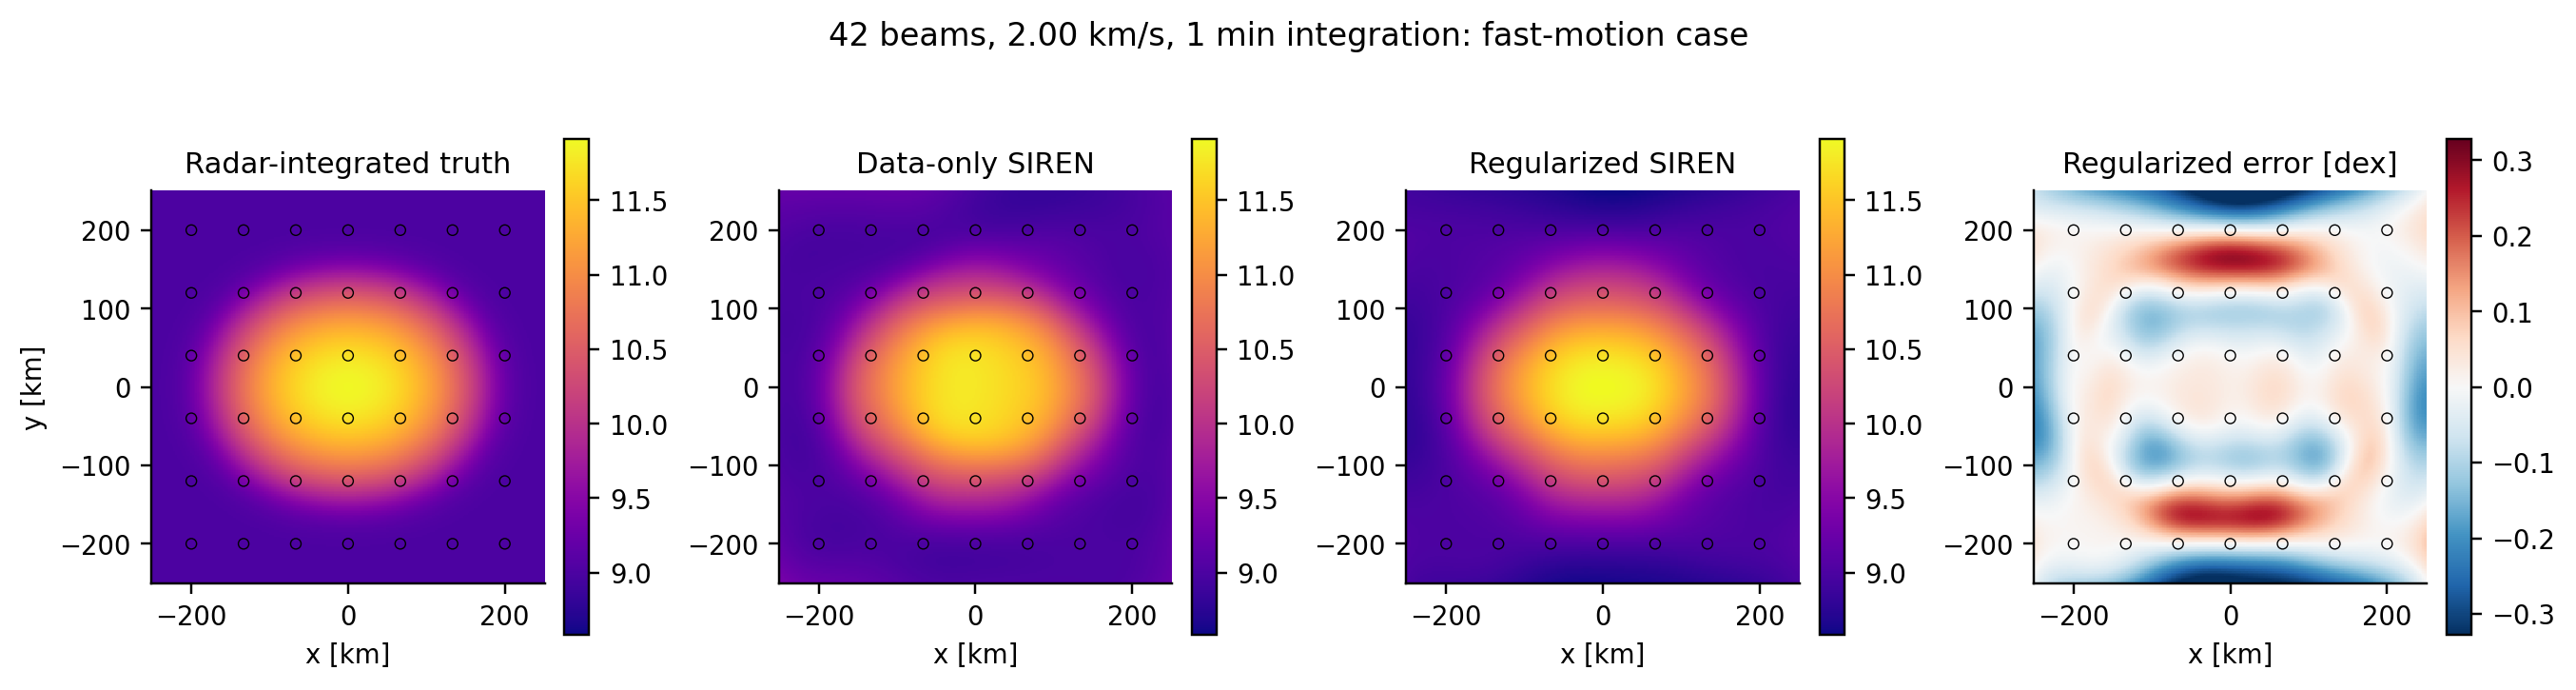
\includegraphics[width=\textwidth]{reconstruction_42_fast_1m.png}
\caption{42 beams, $2.00~\kmps$, 1-minute integration. The represented radar product is recovered with
7.4\% active-region NRMSE under regularization.}
\label{fig:42fast1}
\end{figure}

\subsection{Fast Ten-Minute Radar Product}

Figure~\ref{fig:42fast10} is deliberately described as reconstruction of the radar-integrated target. The
truth is a broad band because that is what the synthetic observation operator supplies. The regularized
model reconstructs it with 5.3\% active NRMSE and 0.999 correlation. This result supports SIREN robustness
for the available product; it is not scored against an instantaneous latent patch.

\begin{figure}[H]
\centering
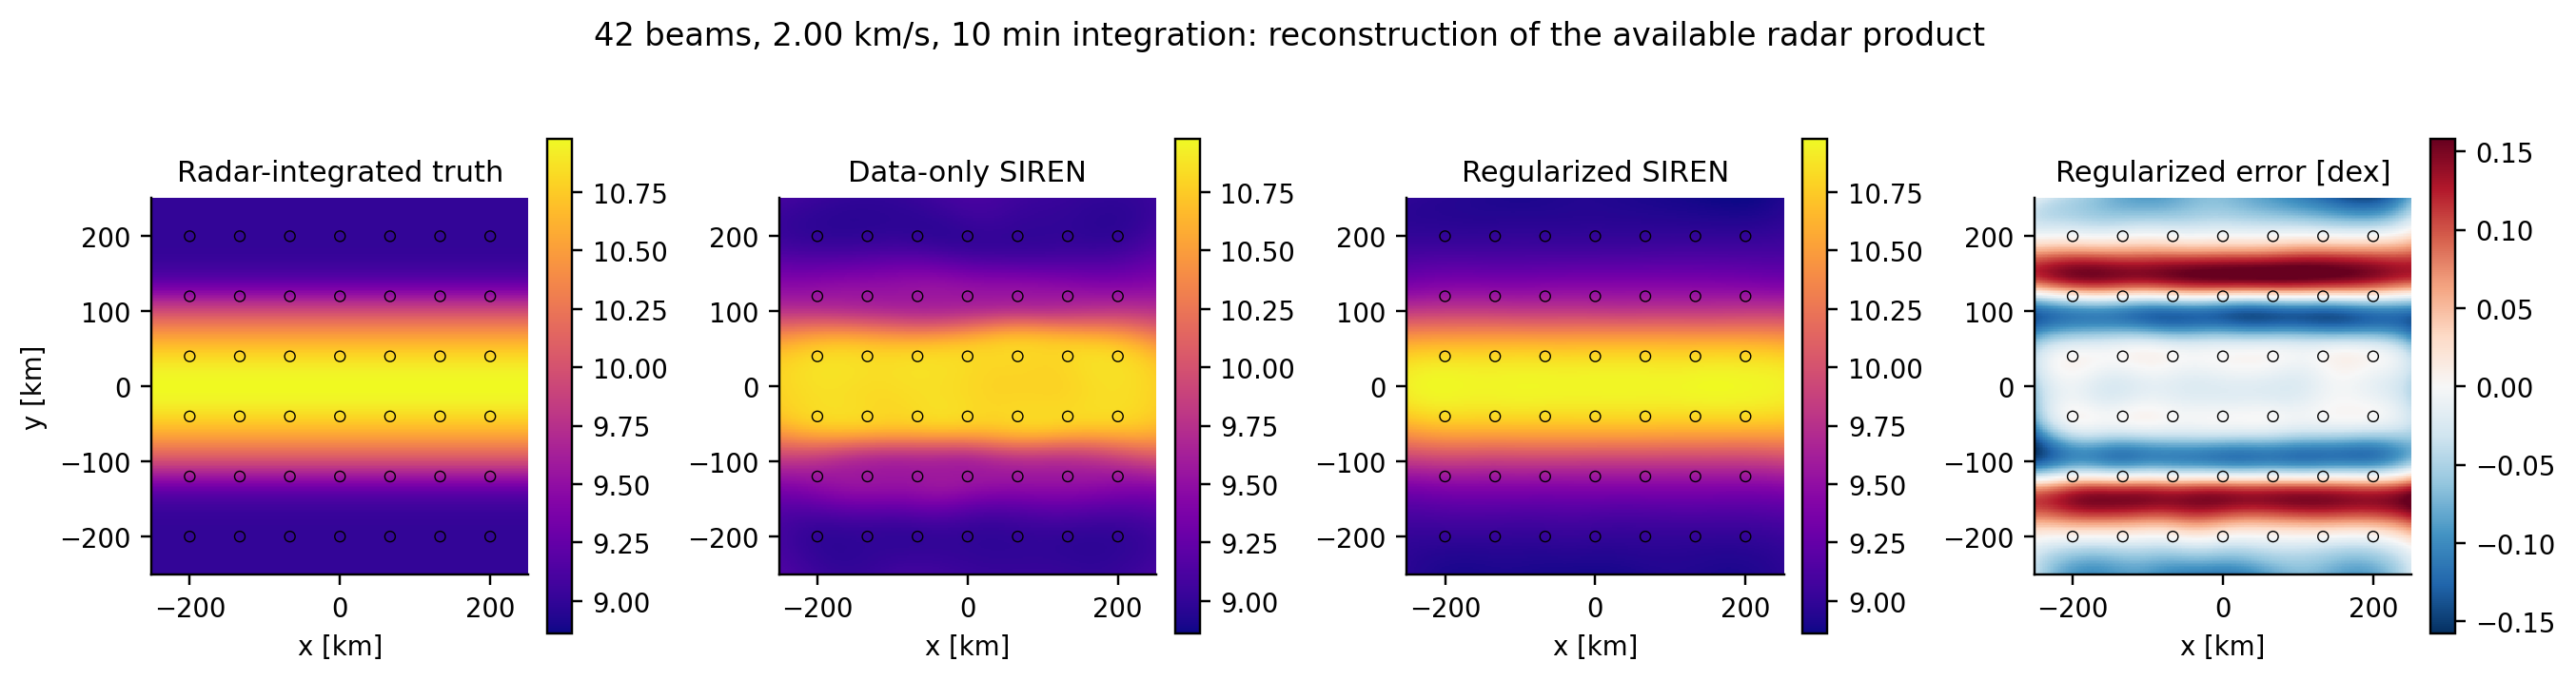
\includegraphics[width=\textwidth]{reconstruction_42_fast_10m.png}
\caption{42 beams, $2.00~\kmps$, 10-minute integration. The broad structure is the radar-integrated
synthetic truth and is therefore the correct reconstruction target.}
\label{fig:42fast10}
\end{figure}

\section{What Synthetic Data Have Established}

The pilot justifies retaining synthetic data, but it also defines their appropriate role.

\subsection{Questions Synthetic Data Answer Well}

\begin{enumerate}
  \item \textbf{Dense interpolation error.} Synthetic truth exists between beams, where real ISR data do not
  provide direct labels.
  \item \textbf{Derivative validation.} Exact spatial and temporal derivatives can be evaluated, making it
  possible to detect an apparently accurate field with incorrect gradients.
  \item \textbf{Failure mechanisms.} Curvature collapse, loss saturation, oversmoothing, unsupported
  oscillations, and support dependence can be isolated.
  \item \textbf{Controlled ablations.} Data-only and regularized models can be compared with identical
  observations, initialization policy, and truth.
  \item \textbf{Reliability truth.} Synthetic tests later permit direct comparison between predicted
  uncertainty and actual reconstruction error.
\end{enumerate}

\subsection{Questions This Pilot Cannot Answer}

\begin{enumerate}
  \item It cannot establish final performance on ISR-derived plasma parameters because the measurements are
  noise free and lack real fitting correlations, quality flags, calibration effects, and systematic errors.
  \item It cannot select final lambda values because all cases use seed zero and no independent validation
  folds.
  \item It cannot establish 4D anisotropy because the current field is horizontal $(x,y,t)$ rather than
  $(x,y,z,t)$.
  \item It cannot calibrate a reliability map without repeated stochastic errors or real held-out residuals.
  \item It cannot establish that SIREN is superior to FINER, Fourier-feature MLPs, K-Planes, Gaussian
  processes, splines, or other baselines \cite{Tancik2020Fourier,Liu2023FINER,FridovichKeil2023KPlanes}.
  \item It cannot represent all auroral morphology with one Gaussian patch and one two-band stress case.
\end{enumerate}

The marginal value of simply expanding the idealized velocity/integration grid is now low. The next synthetic
work should be selected because it answers a specific unresolved question or connects directly to a real-data
experiment.

\section{Recommended Next Synthetic Experiments}

\subsection{Priority 1: Real-Geometry Semi-Synthetic Twin}

The highest-value synthetic extension is not another Cartesian-grid velocity sweep. It is a semi-synthetic
twin of one real ISR experiment. The procedure should be:
\begin{enumerate}
  \item select one real, well-supported 42-beam event with a usable sequence of density, formal uncertainty,
  quality flags, LOS velocity, timestamps, and integration metadata;
  \item preserve the exact sampled coordinates, beam identifiers, missing records, time spacing, and
  altitude/range structure;
  \item evaluate a known continuous plasma field at those real sampling coordinates;
  \item add heteroscedastic errors based on the real $d\Ne$ distribution, with a clearly documented
  systematic floor;
  \item train the same model and evaluate dense truth, withheld beams, withheld times, and reliability.
\end{enumerate}

This experiment bridges the realism gap while retaining known truth. It directly tests whether conclusions
drawn from regular synthetic geometry survive actual radar support. It should be built from the same event
used for the first real-data benchmark so synthetic and real conclusions are comparable.

\subsection{Priority 2: Focused Multi-Seed Regularization Study}

The current 0.30/0.30 setting is consistently better than data only, but a single seed is insufficient for a
final selection. The next regularization study should use four representative cases:
\begin{enumerate}
  \item 42 beams, $0.36~\kmps$, 1 minute: well-supported reference;
  \item 23 beams, $0.36~\kmps$, 1 minute: support-limited interpolation;
  \item 42 beams, $2.00~\kmps$, 1 minute: density-gradient tradeoff;
  \item 23-beam flow reversal, $1.00~\kmps$, 2 minutes: complex morphology.
\end{enumerate}

Use at least three seeds and a compact ratio grid rather than a large arbitrary sweep:
\begin{equation}
  r_{xy}\in\{0,0.10,0.30,0.60\},\qquad
  r_t\in\{0,0.10,0.30,0.60\}.
\end{equation}
Not every Cartesian combination must be run initially. Start with data only, spatial only, temporal only,
0.10/0.10, 0.30/0.30, 0.60/0.30, and 0.30/0.60. Select using a multi-metric validation score that reports
density, gradient, bias, and support-stratified errors separately. An L-curve or Pareto presentation is more
defensible than reducing everything to one opaque scalar \cite{Hansen1992LCurve}.

\subsection{Priority 3: Heteroscedastic and Systematic Error Injection}

The current observations are noise free. The next noise experiment should distinguish:
\begin{description}
  \item[Formal statistical uncertainty.] Draw noise with scale based on empirical real-data $d\Ne$ and use
  the same uncertainty in a heteroscedastic likelihood.
  \item[Beam-dependent calibration offset.] Apply a persistent multiplicative or log-space bias to one or
  more beams. Formal errors alone will not capture this.
  \item[Outliers and quality failures.] Inject a small fraction of grossly corrupted values and compare
  Gaussian, Huber, Cauchy, or quality-masked data terms.
  \item[Missingness.] Remove contiguous beam-time blocks rather than random individual points.
\end{description}

The purpose is not to mimic every ISR systematic effect at once. Each corruption should correspond to a
failure mode that can be identified in residuals and represented in the reliability layer
\cite{LehtinenHuuskonen1996,HuuskonenLehtinen1996,Diaz2026ISRError}.

\subsection{Priority 4: Vertical Structure and Anisotropy}

Before moving to a full 4D real model, create a controlled $(x,y,z,t)$ field with
\begin{equation}
  f(x,y,z,t) = b(z,t) + r(x,y,z,t),
\end{equation}
where $b$ contains a realistic vertical background profile and $r$ contains horizontally moving residual
structure. Include a broad F-region peak, altitude-dependent amplitude, and at least one sharp vertical
transition. This permits separate evaluation of
\begin{equation}
  \lambda_{xy}\mathcal L_{xy} + \lambda_z\mathcal L_z + \lambda_t\mathcal L_t,
\end{equation}
instead of treating $z$ as another horizontal coordinate. The goal is to determine whether the background
plus residual decomposition reduces the burden on SIREN and whether vertical regularization should be robust
or altitude dependent.

\subsection{Priority 5: Morphology Suite}

A small permanent morphology suite should contain:
\begin{enumerate}
  \item one enhancement and one depletion;
  \item two structures crossing or approaching each other;
  \item an elongated arc with a narrow boundary;
  \item the existing flow reversal;
  \item a spatially broad background gradient plus a compact perturbation.
\end{enumerate}
The suite should remain small enough to run routinely after code changes. Its role is regression testing and
architecture ablation, not an attempt to enumerate ionospheric phenomenology.

\begin{table}[H]
\centering
\caption{Recommended synthetic sequence and its decision value.}
\label{tab:syntheticplan}
\small
\begin{tabularx}{\textwidth}{p{0.16\textwidth}p{0.23\textwidth}X p{0.19\textwidth}}
\toprule
Priority & Example & Primary question & Decision criterion \\
\midrule
1 & Real-geometry semi-synthetic twin & Do results survive real coordinates, missingness, timing, and uncertainty? & Agreement between dense truth and held-out residual conclusions \\
2 & Four-case, three-seed lambda study & Is 0.30/0.30 robust and are density/gradient tradeoffs stable? & Pareto stability across seeds and held-out points \\
3 & Heteroscedastic plus systematic errors & Does the likelihood use $d\Ne$ correctly and detect bad beams? & Normalized residuals and outlier robustness \\
4 & 4D vertical-profile plus residual field & What regularization should differ between $xy$ and $z$? & Altitude-stratified density and gradient errors \\
5 & Small morphology regression suite & Which structures expose architecture or prior failure? & Repeatable pass/fail diagnostics after code changes \\
\bottomrule
\end{tabularx}
\end{table}

\section{Recommended Next Real-Data Examples}

\subsection{Immediate Development Event: Well-Supported 42-Beam Sequence}

The next primary example should be one real event with the best available support, not the most spectacular
auroral case. Recommended properties are:
\begin{itemize}
  \item 42-beam or comparably dense geometry;
  \item enough contiguous time records for blocked withheld-time tests;
  \item 1- or 2-minute products if already available, but without treating shorter integration as a model
  quality requirement;
  \item usable $\Ne$, $d\Ne$, LOS velocity, quality flags, elevation, azimuth, range, and altitude;
  \item moderate structure, so implementation failures can be separated from genuinely extreme dynamics.
\end{itemize}

This event should be used to establish the complete real-data evaluation pipeline: coordinate preparation,
heteroscedastic loss, beam/time splitting, baselines, error stratification, and reliability diagnostics.

\subsection{Second Event: Active, Fast, Structurally Complex Interval}

After the pipeline works on the development event, select an active-time event with large LOS velocities and
rapid density structure. The purpose is not to demand recovery of an unobserved instantaneous field. It is to
test whether reconstruction residuals, support diagnostics, and reliability correctly respond when the radar
product changes rapidly and the assumption of a globally smooth field becomes more fragile.

LOS velocity should be introduced cautiously. At first it can support:
\begin{itemize}
  \item event/activity stratification;
  \item reliability features based on displacement over the product interval;
  \item a smoothed horizontal-flow proxy when geometry permits;
  \item optional coordinate conditioning or co-moving-coordinate comparisons.
\end{itemize}
It should not initially be presented as a full vector velocity truth.

\subsection{Third Event: Sparse 11-Beam Reliability Stress Test}

The 11-beam experiment should follow, not precede, the 42-beam development case. Its main success criterion
is not uniformly small reconstruction error. It is whether the system identifies weakly supported regions
and produces appropriately broad or low-confidence reliability estimates. This is where MC dropout plus
geometry/support features or conformal intervals become operationally meaningful
\cite{Gal2016Dropout,AngelopoulosBates2021,Romano2019CQR}.

\subsection{Later Challenge Event: Observed Flow Reversal or Auroral Shear}

If a credible real flow-reversal event is available, it should be treated as a challenge dataset after the
ordinary pipeline is established. The real example should include LOS velocity and sufficient geometry to
support the interpretation. Because the event is rare, it should not dominate model selection; it should
test whether the method reports a plausible field and low reliability where the boundary is unsupported.

\section{Real-Data Validation Protocol}

\subsection{Withheld-Beam Validation}

Random point holdout is too easy because neighboring points from the same beam and time remain available.
Use beam-level folds:
\begin{enumerate}
  \item remove all values from one beam or a geometrically coherent beam group;
  \item train on the remaining beams;
  \item predict the held-out values at their original coordinates and times;
  \item report raw and uncertainty-normalized residuals;
  \item repeat across central, edge, high-elevation, low-elevation, and weak-support beams.
\end{enumerate}

The normalized residual
\begin{equation}
  z_i = \frac{y_i-\widehat y_i}{\sqrt{\sigma_{i,\mathrm{ISR}}^2+\sigma_{\mathrm{model},i}^2}}
\end{equation}
should be analyzed by altitude, SNR, integration product, support distance, and quality flag. Formal ISR errors
are fit uncertainties rather than complete truth errors, so a learned or calibrated systematic floor may be
required \cite{Diaz2026ISRError}.

\subsection{Withheld-Time Validation}

Use contiguous blocks, not isolated random timestamps. Recommended tests include:
\begin{itemize}
  \item one missing interior record;
  \item a short contiguous missing block;
  \item interpolation between two observed blocks;
  \item boundary extrapolation, reported separately from interpolation.
\end{itemize}
For each product, predictions are compared with measurements at that product's own timestamps and integration
definition. No penalty is assigned for failure to infer a hypothetical higher-time-resolution field.

\subsection{Nested Model Selection}

Architecture and lambda selection must not use the final held-out test folds. A defensible hierarchy is:
\begin{enumerate}
  \item training beams/times for parameter fitting;
  \item validation beam/time blocks for lambda and architecture decisions;
  \item untouched test beam/time blocks for final reporting;
  \item conformal calibration data separated from both model training and final coverage evaluation.
\end{enumerate}
Multiple seeds should be reported as distributions, not only best runs.

\subsection{Baselines}

The INR should be compared against methods that answer the same reconstruction question:
\begin{itemize}
  \item nearest-neighbor or piecewise constant interpolation;
  \item linear interpolation or Delaunay-based interpolation where geometry permits;
  \item radial basis functions;
  \item Gaussian-process regression with a documented anisotropic kernel;
  \item temporal smoothing plus spatial interpolation;
  \item data-only SIREN and regularized SIREN.
\end{itemize}
If SIREN does not improve withheld performance or derivative quality over simpler methods, its continuous
field representation may still be useful, but the added complexity must be justified explicitly.

\section{Architecture Decision After Real Validation}

The current results do not justify abandoning SIREN. The baseline is differentiable, trains successfully,
retains nonzero curvature, and reconstructs all ordinary integrated products with good accuracy under
regularization. Architecture comparisons should be triggered by observed failure modes:
\begin{description}
  \item[FINER.] Test if SIREN exhibits spectral-bias or frequency-tuning limitations on narrow arcs or
  multi-scale morphology \cite{Liu2023FINER}.
  \item[Fourier-feature MLP.] Test as a simpler frequency-encoding comparator
  \cite{Tancik2020Fourier}.
  \item[K-Planes or factorized 4D representation.] Test when full $(x,y,z,t)$ memory or training speed becomes
  the bottleneck rather than reconstruction quality \cite{FridovichKeil2023KPlanes}.
  \item[Co-moving or velocity-conditioned coordinates.] Test specifically for fast coherent structures or
  flow-reversal cases when LOS-derived motion information is available.
\end{description}

The comparison must keep the observation target, train/validation splits, parameter budget, and uncertainty
model fixed. Otherwise architecture and data differences will be confounded.

\section{Reliability Map Roadmap}

The final tool should show the reconstructed field and a reliability map together. Reliability is not a
single neural-network variance. It should combine several interpretable components:
\begin{enumerate}
  \item ISR formal uncertainty and quality flags;
  \item distance to the nearest observation and local beam density;
  \item angular diversity and altitude/range support;
  \item withheld-beam and withheld-time residual behavior;
  \item model uncertainty from MC dropout or a learned residual scale;
  \item calibrated conformal interval width and empirical coverage;
  \item warnings for extrapolation and known support gaps.
\end{enumerate}

Integration time may be displayed as measurement metadata and may enter reliability if empirical held-out
errors depend on it. It should not automatically reduce reliability. The relationship must be learned or
validated from the radar products actually being reconstructed.

For conformal prediction, a useful normalized score is
\begin{equation}
  s_i = \frac{|y_i-\widehat y_i|}{\widehat\sigma_i},
\end{equation}
where $\widehat\sigma_i$ may combine ISR uncertainty, MC-dropout scale, and geometry/support features.
Calibration can be group conditioned by altitude, support, elevation, SNR, or experiment type when sample
sizes permit \cite{AngelopoulosBates2021,Romano2019CQR}. The project should report empirical coverage and
interval width together; wide intervals with correct coverage are informative rather than failures.

\section{Recommended Work Sequence}

\begin{table}[H]
\centering
\caption{Recommended project sequence after this pilot.}
\label{tab:sequence}
\small
\begin{tabularx}{\textwidth}{p{0.08\textwidth}p{0.23\textwidth}X p{0.22\textwidth}}
\toprule
Stage & Deliverable & Main work & Gate before proceeding \\
\midrule
1 & Real-data development benchmark & One 42-beam event, data model, $d\Ne$ loss, withheld beams/times, simple baselines & Reproducible held-out metrics and no split leakage \\
2 & Semi-synthetic twin & Same geometry/timing/errors with known dense truth & Synthetic dense error agrees qualitatively with held-out rankings \\
3 & Focused regularization study & Four cases, at least three seeds, compact ratio grid, lambda-cap test & Stable Pareto choice across seeds and density/gradient metrics \\
4 & Reliability prototype & Geometry/support map plus MC dropout or conformal calibration & Coverage and interval width reported on untouched folds \\
5 & Sparse and active challenges & 11-beam event, fast active event, later flow reversal & Reliability degrades appropriately where support is weak \\
6 & Architecture ablation & SIREN versus FINER/Fourier; K-Planes only for 4D scaling & Alternative wins held-out metrics or computational cost materially \\
\bottomrule
\end{tabularx}
\end{table}

The immediate next example should therefore be:
\begin{quote}
\textbf{One well-supported real 42-beam ISR event, paired with a semi-synthetic twin using its exact geometry,
timestamps, integration products, formal errors, missingness, and quality metadata.}
\end{quote}

This pair answers more unresolved questions than another broad idealized synthetic sweep. The real event
tests operational reconstruction and held-out generalization. The semi-synthetic twin provides dense truth
and derivative diagnostics. Together they determine whether the current SIREN and regularization behavior
transfer to realistic radar support.

\section{Conclusions}

The 18-run pilot supports continued use of the regularized SIREN baseline. Against the correct target---the
radar-integrated synthetic field---\targetreg{} improves active-region density reconstruction in every case,
reduces error by 49.2\% on average, and yields 4.7\%--7.4\% NRMSE for the four ordinary 42-beam cases. The
23-beam cases are less accurate but remain usable at 12.4\%--17.3\%. The dominant limitation is observation
support, not integration time or a demonstrated SIREN incapacity.

The flow-reversal case shows that the method can recover broad two-band morphology but not fully resolve the
boundary from sparse density samples alone. LOS velocity is the appropriate next source of information for
that problem. Curvature diagnostics confirm that no model collapsed, but the temporal-lambda ceiling prevents
10-minute cases from attaining the requested 0.30 loss ratio. That controller issue should be studied in a
focused, multi-seed experiment rather than through indiscriminate cap increases.

Synthetic data should remain a permanent diagnostic asset, especially for derivatives, failure modes, and
reliability truth. It should no longer be the project's primary evidence. The next milestone is real held-out
validation, paired with a real-geometry semi-synthetic twin. Architecture changes should follow only if that
validation identifies a failure that SIREN regularization cannot resolve.

\appendix

\section{Reproducibility and Output Inventory}

The pilot output root is
\begin{verbatim}
/home/jdiaz/postdoc/codex-inr-radar/inf_fakedata_3d/
  outputs/velocity_integration_benchmark/
\end{verbatim}
The principal machine-readable summaries are:
\begin{itemize}
  \item \texttt{benchmark\_manifest.csv}: factor settings and run directories;
  \item \texttt{benchmark\_metrics.csv}: first/middle/last dense summaries;
  \item \texttt{benchmark\_event\_summary.csv}: central event-aware metrics;
  \item \texttt{benchmark\_regularization\_comparison.csv}: paired improvements;
  \item \texttt{curvature\_health.csv}: derivative-collapse checks;
  \item each run's \texttt{history.csv}, checkpoint, dense CSVs, and error maps.
\end{itemize}

The event-aware summary is generated by
\texttt{summarize\_velocity\_integration\_results.py}. Figures in this report are generated by the included
\texttt{make\_results\_figures.py}. The analysis uses physical linear-density errors after converting network
predictions from $\log_{10}\Ne$ to $\Ne$; log-space metrics are retained separately.

\section{Interpretive Limitations}

\begin{enumerate}
  \item All pilot cases use one seed. Reported improvements are observed effect sizes, not confidence
  intervals.
  \item Ordinary one-minute dense analysis currently emphasizes first, middle, and last records. The event
  summary corrects the empty-background issue by using the middle active frame, but an all-active-time summary
  should be added for the final synthetic paper.
  \item The synthetic beam patterns approximate support counts but are not exact ISR experiment geometries.
  \item The synthetic data are noise free. The strong measured-point fit is therefore expected and does not
  represent real ISR residual structure.
  \item The current model is $(x,y,t)$ at a selected altitude context, not full $(x,y,z,t)$.
  \item The flow-reversal case is a constructed two-band density example. It is not a full electrodynamic
  simulation and does not establish vector velocity reconstruction.
  \item Results should not be generalized to $\Te$, $\Ti$, or LOS velocity without parameter-specific error
  and prior studies.
\end{enumerate}

\begin{thebibliography}{99}

\bibitem{Diaz2026Proposal}
J. Diaz Pena.
\newblock \emph{Uncertainty-Aware AI to Reconstruct 4D Ionospheric Structure from Sparse Multi-Beam Radar Data}.
\newblock UAI PostDoc proposal, 2026.

\bibitem{Diaz2026ISRError}
J. Diaz Pena.
\newblock \emph{The Physics and Mathematics of Uncertainty in Incoherent Scatter Radar Data: An Analysis of AMISR Fitting Processes and Error Propagation}.
\newblock Internal project report, 2026.

\bibitem{Sitzmann2020SIREN}
V. Sitzmann, J. N. P. Martel, A. W. Bergman, D. B. Lindell, and G. Wetzstein.
\newblock Implicit neural representations with periodic activation functions.
\newblock \emph{Advances in Neural Information Processing Systems}, 2020.
\newblock \url{https://arxiv.org/abs/2006.09661}

\bibitem{Tancik2020Fourier}
M. Tancik et al.
\newblock Fourier features let networks learn high frequency functions in low dimensional domains.
\newblock \emph{Advances in Neural Information Processing Systems}, 2020.
\newblock \url{https://arxiv.org/abs/2006.10739}

\bibitem{Liu2023FINER}
Z. Liu et al.
\newblock FINER: Flexible spectral-bias tuning in implicit neural representation by variable-periodic activation functions.
\newblock arXiv:2312.02434, 2023.
\newblock \url{https://arxiv.org/abs/2312.02434}

\bibitem{FridovichKeil2023KPlanes}
S. Fridovich-Keil, G. Meanti, F. Warburg, B. Recht, and A. Kanazawa.
\newblock K-Planes: Explicit radiance fields in space, time, and appearance.
\newblock \emph{CVPR}, 2023.
\newblock \url{https://arxiv.org/abs/2301.10241}

\bibitem{LehtinenHuuskonen1996}
M. S. Lehtinen and A. Huuskonen.
\newblock General incoherent scatter analysis and GUISDAP.
\newblock \emph{Journal of Atmospheric and Terrestrial Physics}, 58(1--4):435--452, 1996.

\bibitem{HuuskonenLehtinen1996}
A. Huuskonen and M. S. Lehtinen.
\newblock The accuracy of incoherent scatter measurements: error estimates valid for high signal levels.
\newblock \emph{Journal of Atmospheric and Terrestrial Physics}, 58(1--4):453--463, 1996.

\bibitem{Virtanen2008}
I. I. Virtanen, M. S. Lehtinen, T. Nygren, M. Orispaa, and M. Vierinen.
\newblock A Bayesian approach to incoherent scatter radar analysis.
\newblock \emph{Annales Geophysicae}, 26:571--586, 2008.

\bibitem{Hansen1992LCurve}
P. C. Hansen.
\newblock Analysis of discrete ill-posed problems by means of the L-curve.
\newblock \emph{SIAM Review}, 34(4):561--580, 1992.

\bibitem{Chen2018GradNorm}
Z. Chen, V. Badrinarayanan, C.-Y. Lee, and A. Rabinovich.
\newblock GradNorm: Gradient normalization for adaptive loss balancing in deep multitask networks.
\newblock \emph{International Conference on Machine Learning}, 2018.
\newblock \url{https://arxiv.org/abs/1711.02257}

\bibitem{Heydari2019SoftAdapt}
A. A. Heydari, C. A. Thompson, and A. Mehmood.
\newblock SoftAdapt: Techniques for adaptive loss weighting of neural networks with multi-part loss functions.
\newblock arXiv:1912.12355, 2019.
\newblock \url{https://arxiv.org/abs/1912.12355}

\bibitem{Kendall2018MultiTask}
A. Kendall, Y. Gal, and R. Cipolla.
\newblock Multi-task learning using uncertainty to weigh losses for scene geometry and semantics.
\newblock \emph{CVPR}, 2018.
\newblock \url{https://arxiv.org/abs/1705.07115}

\bibitem{Gal2016Dropout}
Y. Gal and Z. Ghahramani.
\newblock Dropout as a Bayesian approximation: Representing model uncertainty in deep learning.
\newblock \emph{International Conference on Machine Learning}, 2016.
\newblock \url{https://arxiv.org/abs/1506.02142}

\bibitem{AngelopoulosBates2021}
A. N. Angelopoulos and S. Bates.
\newblock A gentle introduction to conformal prediction and distribution-free uncertainty quantification.
\newblock arXiv:2107.07511, 2021.
\newblock \url{https://arxiv.org/abs/2107.07511}

\bibitem{Romano2019CQR}
Y. Romano, E. Patterson, and E. J. Candes.
\newblock Conformalized quantile regression.
\newblock \emph{Advances in Neural Information Processing Systems}, 2019.
\newblock \url{https://arxiv.org/abs/1905.03222}

\end{thebibliography}

\end{document}
